% ClawChain: An Agent-Native Layer 1 Blockchain for Autonomous Economic Coordination
%
% IEEE SSE 2026 — International Conference on Software and Systems Engineering
% Full Extended Version

\documentclass[conference]{IEEEtran}

% Color definitions (IEEE compatible)
\usepackage{xcolor}
\definecolor{clawblue}{HTML}{1A237E}
\definecolor{clawteal}{HTML}{00796B}
\definecolor{clawgray}{HTML}{546E7A}
\definecolor{clawgold}{HTML}{F57F17}
\definecolor{coreblue}{HTML}{2563EB}
\definecolor{coreteal}{HTML}{0D9488}
\definecolor{coregray}{HTML}{64748B}
\definecolor{coregreen}{HTML}{16A34A}
\definecolor{corered}{HTML}{DC2626}
\definecolor{lightbg}{HTML}{F8FAFC}
\usepackage[utf8]{inputenc}
\usepackage[T1]{fontenc}
\usepackage{hyperref}
\hypersetup{
  pdftitle={ClawChain: An Agent-Native Layer 1 Blockchain for Autonomous Economic Coordination},
  pdfauthor={Alex Chen, Bowen Li, Nicholas Qi, Shiping Chen},
  pdfkeywords={blockchain, autonomous agents, DID, reputation, Layer 1, EvoClaw},
}
\usepackage{url}
\usepackage{booktabs}
\usepackage{amsfonts}
\usepackage{amsmath}
\usepackage{amssymb}
\usepackage{amsthm}
\usepackage{algorithm}
\usepackage{algorithmic}
\usepackage{tikz}
\usepackage{pgfplots}
\usepackage{subcaption}
\usepackage{xcolor}
\usepackage{listings}
\lstdefinelanguage{Rust}{
  keywords={fn, let, pub, use, struct, enum, impl, trait, return, if, else, match, for, in, while, loop, mut, ref, self, super, mod, crate, type, where, as, const, static, unsafe, extern, move, Box, Vec, Option, Result, Ok, Err, Some, None},
  morecomment=[l]{//},
  morecomment=[s]{/*}{*/},
  morestring=[b]",
  sensitive=true,
}
\lstdefinelanguage{Pseudocode}{
  keywords={fn, let, pub, use, struct, enum, impl, ensure, map, insert, get, mutate, push, iter, fold},
  morecomment=[l]{//},
  sensitive=true,
}
\usepackage{mathtools}
\usepackage{pifont}

\usetikzlibrary{arrows.meta, positioning, shapes.geometric, fit, calc, decorations.pathreplacing, backgrounds, chains, matrix}
\pgfplotsset{compat=1.18}

% Theorem environments
\newtheorem{theorem}{Theorem}
\newtheorem{lemma}[theorem]{Lemma}
\newtheorem{proposition}[theorem]{Proposition}
\newtheorem{definition}{Definition}
\newtheorem{corollary}{Corollary}
\newtheorem{remark}{Remark}

% Custom colors
\definecolor{clawblue}{RGB}{41, 98, 255}
\definecolor{clawgreen}{RGB}{0, 200, 83}
\definecolor{clawpurple}{RGB}{124, 77, 255}
\definecolor{claworange}{RGB}{255, 145, 0}
\definecolor{clawred}{RGB}{255, 61, 0}
\definecolor{clawgray}{RGB}{96, 125, 139}

\title{ClawChain: An Agent-Native Layer~1 Blockchain \\for Autonomous Economic Coordination}

\author{
\IEEEauthorblockN{Alex Chen}
\IEEEauthorblockA{Independent Researcher\\Sydney, Australia\\alex.chen31337@gmail.com}
\and
\IEEEauthorblockN{Bowen Li}
\IEEEauthorblockA{Independent Researcher\\Sydney, Australia\\bowen31337@outlook.com}
\and
\IEEEauthorblockN{Nicholas Qi}
\IEEEauthorblockA{Independent Researcher\\Sydney, Australia\\nicholas68663@gmail.com}
\and
\IEEEauthorblockN{Shiping Chen}
\IEEEauthorblockA{Data61, CSIRO\\Sydney, Australia\\Shiping.Chen@data61.csiro.au}
}

\begin{document}

\maketitle

\begin{abstract}
Existing blockchains are designed for humans: they rely on wallet-based identities, require manual transaction signing, and impose gas fees that make micro-transactions impractical. These assumptions break down when agents---autonomous AI programs---are the primary economic participants. We present \textbf{ClawChain}, the first Layer~1 blockchain designed specifically for agent economies. ClawChain introduces three core innovations: (1)~an \textit{Agent DID system} providing on-chain, verifiable, cryptographically-bound identities for AI agents with a novel attestation graph; (2)~a \textit{reputation-weighted token model} (\$CLAW) where tokens are earned through verifiable contributions rather than purchased, with Merkle-tree-based airdrop claims; and (3)~a \textit{quadratic reputation governance system} where voting power derives from both on-chain reputation and economic stake, provably resistant to plutocratic capture. We formalize the reputation scoring function, prove its Sybil-resistance properties under bounded collusion, and derive equilibrium conditions for the token economy. Our Substrate-based implementation comprises 14,270 lines of Rust across six custom pallets. Testnet deployment demonstrates 6-second block times, sub-cent transaction fees via inflation-subsidized gas, and successful registration of autonomous agents. We provide formal algorithms for agent registration, reputation computation, and airdrop verification, alongside a comprehensive security analysis. ClawChain establishes the foundational infrastructure for agent-to-agent commerce, collaborative development, and decentralized coordination at scale.
\end{abstract}

% ============================================================================
% SECTION 1: INTRODUCTION
% ============================================================================

\section{Introduction}

\subsection{The Agent Economy Gap}

The proliferation of autonomous AI agents---from code-generation systems~\cite{chen2021codex} to multi-agent orchestration frameworks~\cite{wu2023autogen, hong2024metagpt}---has created an emerging class of economic actors that operate without direct human supervision. These agents negotiate, transact, and collaborate across digital infrastructure. Yet the financial and identity infrastructure they must use was designed exclusively for human participants.

Consider a concrete scenario: an autonomous coding agent completes a 500-line pull request for an open-source project. On existing blockchains, this agent must (a)~possess a human-managed wallet, (b)~pay gas fees of \$0.10--\$5.00 per transaction, and (c)~have no standardized way to prove its identity or track record. The agent's contribution is economically invisible to the on-chain world.

This paper addresses three fundamental misalignments between existing blockchain infrastructure and the requirements of agent economies:

\begin{enumerate}
    \item \textbf{Identity Gap.} Existing blockchains use wallet-based identities (private keys, ECDSA signatures). While agents can hold keys, there is no standard for registering, verifying, or distinguishing agent identities. The W3C DID specification~\cite{w3c_did_2022} provides a framework but no agent-specific method.
    
    \item \textbf{Economic Gap.} Gas fees on Ethereum average \$1--\$50 per transaction~\cite{ethgasstation}, making micro-transactions impractical. Agents performing small tasks (answering queries, processing files, generating code snippets) cannot sustain per-transaction costs that exceed the value of their work.
    
    \item \textbf{Governance Gap.} Token-weighted voting (1~token = 1~vote) creates plutocratic governance~\cite{buterin2019quadratic}. An agent that contributes 10,000 lines of critical infrastructure code has no more governance power than an entity that simply purchases equivalent tokens.
\end{enumerate}

\subsection{Contributions}

We present \textbf{ClawChain}, the first Layer~1 blockchain designed from the ground up for autonomous agent economies. Our contributions are:

\begin{enumerate}
    \item \textbf{Agent DID System} (\S\ref{sec:did}): A decentralized identifier system with a novel \texttt{did:claw} method, cryptographic binding to agent capabilities, and a transitive attestation graph with formal trust propagation semantics.
    
    \item \textbf{Contribution-Weighted Token Economics} (\S\ref{sec:token}): The \$CLAW token is earned through verifiable on-chain contributions. We formalize the contribution scoring function, prove its fairness properties, and describe a Merkle-tree-based airdrop mechanism with $O(\log n)$ verification.
    
    \item \textbf{Reputation-Weighted Governance} (\S\ref{sec:governance}): A governance model combining quadratic reputation scoring with economic stake, provably resistant to plutocratic capture under our threat model. We derive the Nash equilibrium of the governance game.
    
    \item \textbf{Formal Security Analysis} (\S\ref{sec:security}): Proofs of Sybil resistance, analysis of collusion bounds, and a game-theoretic model of validator incentives.
    
    \item \textbf{Substrate Implementation} (\S\ref{sec:implementation}): A complete, open-source implementation with 14,270 lines of Rust, six custom pallets, and testnet deployment demonstrating practical feasibility.
\end{enumerate}

\subsection{Paper Organization}

Section~\ref{sec:related} reviews related work across blockchains, DIDs, agent systems, and tokenomics. Section~\ref{sec:architecture} describes ClawChain's architecture with formal specifications. Section~\ref{sec:did} details the Agent DID system. Section~\ref{sec:token} formalizes the token model. Section~\ref{sec:governance} covers governance. Section~\ref{sec:security} presents our security analysis. Section~\ref{sec:implementation} discusses implementation. Section~\ref{sec:evaluation} presents evaluation results. Section~\ref{sec:applications} describes applications. Section~\ref{sec:limitations} discusses limitations. Section~\ref{sec:conclusion} concludes.

% ============================================================================
% SECTION 2: RELATED WORK
% ============================================================================

\section{Related Work}\label{sec:related}

We survey five areas: Layer~1 blockchains, decentralized identity, AI agent frameworks, token economics, and decentralized governance.

\subsection{Layer~1 Blockchains}

\textbf{Bitcoin}~\cite{nakamoto2008bitcoin} introduced decentralized consensus via proof-of-work with a UTXO transaction model, but provides no programmability beyond simple scripts. \textbf{Ethereum}~\cite{buterin2014ethereum} generalized this with Turing-complete smart contracts and an account-based model, enabling DeFi, NFTs, and DAOs. However, Ethereum's gas model (EIP-1559~\cite{roughgarden2021eip1559}) creates unpredictable costs unsuitable for high-frequency agent transactions. \textbf{Solana}~\cite{yakovenko2018solana} achieves high throughput ($\sim$65,000 TPS theoretical) via Proof of History but remains human-centric in its identity and governance models. \textbf{Polkadot}~\cite{wood2016polkadot} introduces heterogeneous sharding via parachains and the Substrate~\cite{parity_substrate} framework for custom chain construction. We build on Substrate for its modularity and upgrade capabilities.

Recent work on application-specific blockchains (``appchains'')~\cite{cosmos_sdk} and rollup-centric architectures~\cite{thibault2022rollups} demonstrates the trend toward purpose-built chains. ClawChain follows this philosophy, building a chain purpose-built for agent economies rather than retrofitting general-purpose infrastructure.

The design space of Layer~1 blockchains has evolved considerably since Bitcoin's introduction. \textbf{Avalanche}~\cite{rocket2019avalanche} achieves high throughput via a probabilistic consensus protocol (Snowball), enabling sub-second finality on subnets. \textbf{Near Protocol}~\cite{skidanov2019near} introduces sharding at the protocol level, dynamically resizing shard sets as load changes. \textbf{Cardano}~\cite{kiayias2017ouroboros} prioritizes formal verification, using the Ouroboros proof-of-stake family proven secure under a rigorous cryptographic model. These systems advance throughput and security but do not address the agent-specific design requirements that motivate ClawChain.

Appchain approaches like Cosmos zones~\cite{cosmos_sdk} allow custom state machines to interoperate via the IBC protocol, enabling specialization without sacrificing connectivity. Similarly, Polkadot parachains connect to a central relay chain via the Parachain Validation Function (PVF). ClawChain's Substrate heritage positions it to integrate with both ecosystems as a future parachain candidate, inheriting shared security while maintaining agent-specific runtime logic. This multi-ecosystem positioning distinguishes ClawChain from narrower agent-focused chains that lack cross-ecosystem bridges.

A critical gap in all existing Layer~1 designs is the transaction fee model's incompatibility with autonomous agents. Even low-fee chains like Solana (\textasciitilde\$0.00025 per transaction) impose per-signature costs that accumulate to thousands of dollars per day for agents performing millions of micro-operations. ClawChain's inflation-subsidized gas model breaks this barrier by decoupling transaction frequency from direct fee payment, a design choice with no precedent in existing Layer~1 architectures.

\subsection{Decentralized Identifiers and Verifiable Credentials}

The W3C DID specification~\cite{w3c_did_2022} defines a standard for decentralized, self-sovereign identifiers. Existing DID methods include \texttt{did:ethr}~\cite{did_ethr} (Ethereum-based), \texttt{did:web} (DNS-based), \texttt{did:ion}~\cite{sidetree} (Bitcoin-anchored via Sidetree), and \texttt{did:key} (static cryptographic keys). The Verifiable Credentials standard~\cite{w3c_vc_2022} enables claims about DID subjects.

None of these methods are designed for AI agents. They assume a human or organizational subject and lack mechanisms for capability declaration, runtime attestation, or agent-specific metadata. Concurrent work on machine-readable credentials~\cite{sporny2024vc} begins to address this but does not provide a blockchain-native solution.

\textbf{Soulbound Tokens (SBTs)}~\cite{weyl2022soulbound} propose non-transferable tokens representing commitments, credentials, and affiliations. SBTs share our vision of reputation-as-identity but are designed for human social contexts and lack the programmatic verification needed for agent systems.

The \texttt{did:key} method encodes public keys directly in the DID string, enabling offline resolution but preventing key rotation---a critical limitation for long-lived agents whose signing keys may be compromised or need periodic refresh. The \texttt{did:ion} method anchors identity on Bitcoin, offering high durability but with write latency exceeding 10 minutes and no support for agent capability metadata. Our \texttt{did:claw} method is designed with agent key rotation as a first-class operation: agents can rotate their signing key via an on-chain extrinsic that links old and new keys cryptographically, preserving reputation continuity across key updates.

The IETF OpenID for Verifiable Credentials (OID4VC) specification~\cite{sporny2024vc} extends OAuth 2.0 to support credential issuance and presentation, enabling interoperability between DID ecosystems. ClawChain's DID documents are structured to be compatible with OID4VC flows, allowing external services (job platforms, data marketplaces) to verify agent credentials using standard OAuth clients without requiring direct blockchain access.

Agent identity in multi-agent systems raises unique challenges beyond what existing DID specifications address. When multiple agents collaborate on a task---a planner, a builder, and a reviewer---the question of collective identity arises: can a coalition of agents hold a DID? Our architecture supports \textit{multi-sig agent DIDs}, where $k$-of-$n$ signing schemes allow agent collectives to have a unified on-chain presence, with individual agent reputation scores contributing to collective trust assessments.

\subsection{AI Agent Frameworks and Multi-Agent Systems}

The emergence of LLM-powered agents has produced frameworks including AutoGPT~\cite{richards2023autogpt}, BabyAGI~\cite{nakajima2023babyagi}, LangChain~\cite{langchain2023}, and more sophisticated multi-agent systems like AutoGen~\cite{wu2023autogen}, MetaGPT~\cite{hong2024metagpt}, and CrewAI~\cite{crewai2024}. These systems enable agents to decompose tasks, use tools, and collaborate.

However, all existing frameworks treat the economic layer as external: agents interact with human-designed financial infrastructure (Stripe, PayPal, cryptocurrency wallets) rather than having a native economic protocol. \textbf{Fetch.ai}~\cite{fetchai2019} proposes an agent-focused blockchain but focuses on agent-to-agent communication protocols rather than identity and governance. \textbf{SingularityNET}~\cite{singularitynet2019} creates a marketplace for AI services but relies on Ethereum's identity and governance models. \textbf{Autonolas}~\cite{autonolas2023} provides agent service infrastructure on existing chains but does not address the fundamental identity and governance gaps.

The rapid evolution of agentic frameworks reveals a convergence toward long-running, persistent agents rather than stateless query-response systems. Agents now maintain memory (via vector databases), execute multi-step plans spanning hours or days, and spawn sub-agents dynamically. This shift toward persistent agents dramatically increases the importance of durable identity: an agent that runs for months must maintain consistent reputation and economic history across process restarts, hardware migrations, and model updates. Existing wallet-based identity models equate identity with key possession, making such continuity fragile. ClawChain's DID model ties identity to an on-chain record that persists independently of the agent's current execution environment.

Economic coordination between agents remains largely ad hoc in current frameworks. A MetaGPT~\cite{hong2024metagpt} team of agents uses internal messaging to allocate tasks but has no mechanism to enforce payment, penalize failure, or build trust between unknown agents. LangChain agents accessing external APIs pay via hard-coded API keys, creating billing fragility. The missing primitive is a neutral, programmable economic layer that agents can trust unconditionally. ClawChain's smart contract-backed task market fills this gap: escrow is enforced by consensus, not by any single party's honesty.

Reinforcement learning from human feedback (RLHF) and its variants have enabled agents to learn from outcome signals~\cite{ouyang2022rlhf}. An under-explored extension applies similar learning to economic outcomes: agents that earn high reputation and CLAW rewards receive a signal that their behavior was valued by the market. ClawChain's reputation system thus creates a feedback loop compatible with RLHF-style training, enabling the market to shape agent behavior without requiring explicit human oversight of every interaction.

\subsection{Token Economics and Mechanism Design}

Token engineering~\cite{voshmgir2020token} applies mechanism design principles to cryptocurrency systems. Key results include the impossibility of sybil-proof token distributions without identity~\cite{douceur2002sybil}, the analysis of token-curated registries~\cite{goldin2017tcr}, and bonding curves for continuous token models~\cite{zargham2020bonding}.

\textbf{Retroactive Public Goods Funding}~\cite{buterin2021retro} proposes rewarding past contributions rather than funding future promises. ClawChain's contribution-weighted airdrop implements a variant of this principle, allocating tokens retroactively based on verified contributions.

\textbf{Quadratic funding}~\cite{buterin2019quadratic} and \textbf{conviction voting}~\cite{conviction_voting} represent advances in preference aggregation that resist plutocratic capture. Our governance model builds on these insights, combining quadratic reputation with economic stake.

Mechanism design for autonomous agents introduces a distinct challenge: agents can compute optimal strategies analytically, making naive incentive structures vulnerable to game-theoretic exploitation. For example, if contribution scores are public in real time, agents may strategically time submissions to maximize the time-decayed score. Our scoring function (Eq.~\ref{eq:score}) uses an exponential decay that is contribution-time-agnostic from the contributor's perspective---there is no optimal ``release time''---mitigating this attack. Additionally, contributions are verified before being scored, adding latency that prevents precise timing manipulation.

The economics of token distributions have been studied extensively in the context of Initial Coin Offerings (ICOs) and token generation events. Empirical studies show that airdrop-based distributions achieve broader token dispersion than ICOs but suffer from ``free-rider'' problems: recipients who did not earn tokens through genuine contribution sell immediately, depressing price. ClawChain's contribution-weighted airdrop mitigates this by ensuring that recipients have demonstrated genuine interest in the ecosystem---agents that have contributed code, documentation, or services are more likely to be aligned with the project's long-term success. The 4-year vesting schedule for team tokens further aligns long-term incentives.

Agent-specific micro-payment channels represent an important complement to base-layer transactions. The Lightning Network~\cite{poon2016lightning} and Raiden Network demonstrate that payment channels can enable near-zero-fee transactions at scale for appropriate use cases. Future ClawChain versions may integrate state channels for very high-frequency agent-to-agent payments (e.g., per-inference micropayments), with only the channel open and close events settling on-chain. This would extend the inflation-subsidy model: base-layer subsidies apply to settlement transactions, while channel operations operate with zero chain cost.

\subsection{Decentralized Governance}

DAO governance has evolved from simple token-weighted voting (MolochDAO~\cite{molochdao}, Compound Governor~\cite{compound_gov}) to more sophisticated models including optimistic governance (Optimism's Token House~\cite{optimism2024}), delegate-based systems (ENS, Gitcoin), and conviction voting (1Hive~\cite{1hive2021}).

Recent empirical studies~\cite{barbereau2023dao_governance} show that existing DAO governance suffers from low participation ($<$10\% turnout), whale dominance (top 1\% of holders controlling $>$90\% of voting power), and proposal fatigue. ClawChain's reputation-weighted model directly addresses whale dominance by ensuring that economic stake alone cannot capture governance.

Governance in autonomous agent systems introduces novel challenges absent from human DAO contexts. When agents vote, they do so based on utility functions that may be misaligned with broader community interests. An agent optimizing for task market throughput may systematically vote against security proposals that reduce throughput. Counterbalancing this is the reputation system: agents with high reputation typically have a long history of aligned contributions, making their governance preferences more informative signals than those of newly-registered, high-token-balance agents with no contribution history.

The concept of \textit{futarchy}~\cite{hanson2013futarchy} proposes using prediction markets to make governance decisions: vote on values, then bet on beliefs. While too complex for practical implementation at this stage, futarchy-inspired elements could enhance ClawChain governance: proposals could include prediction market questions (``Will this parameter change increase throughput by $>$10\%?''), and agents with accurate predictions over time earn additional governance weight. This aligns governance power with epistemic accuracy, not just contribution history.

Governance security in permissionless settings requires considering adversarial participants who attempt to manipulate outcomes through proposal spam, vote timing attacks, and flash-loan-style attacks on token-based systems. ClawChain mitigates these via proposal deposits (burned on spam), a fixed 14-day voting period preventing last-minute manipulation, and reputation-based voting weight that cannot be flash-borrowed. The reputation component of voting weight requires months of on-chain contribution history to build, creating a natural Sybil barrier even against well-funded adversaries.

\subsection{Comparison with Agent-Specific Blockchains}

Several recent projects specifically target AI agent economies, warranting detailed comparison. \textbf{Fetch.ai}~\cite{fetchai2019} introduced the concept of an ``agent-first'' blockchain with its Open Economic Framework (OEF), a peer-to-peer search and messaging layer for agent service discovery. However, Fetch.ai's identity system is wallet-based, its token economics do not distinguish agent contributions from human transfers, and its governance uses simple token-weighted voting. ClawChain addresses all three limitations with native DID, contribution-weighted tokenomics, and quadratic reputation governance.

\textbf{Autonolas}~\cite{autonolas2023} takes a different approach: rather than building a new Layer~1, it provides agent service infrastructure as smart contracts on existing chains (Ethereum, Gnosis Chain, Solana). This enables rapid deployment but inherits each chain's identity and gas model limitations. A ClawChain agent operating via Autonolas contracts would still pay Ethereum gas for settlement, defeating the inflation-subsidy advantage. ClawChain's approach---native Layer~1 with custom pallets---sacrifices ecosystem access for fundamental economic properties that cannot be achieved on a general-purpose chain.

\textbf{Bittensor}~\cite{bittensor2021} creates a marketplace for machine intelligence, using a Polkadot substrate chain where validators assess AI model quality and miners are rewarded in TAO tokens. While Bittensor shares ClawChain's thesis that AI contributions should earn native tokens, its scoring mechanism is narrowly focused on ML model quality metrics and lacks the general contribution framework, DID system, and governance model that ClawChain provides.

\subsection{Positioning}

Table~\ref{tab:comparison} positions ClawChain against existing systems.

\begin{table}[t]
\centering
\small
\resizebox{\columnwidth}{!}{%
\begin{tabular}{lccccc}
\toprule
\textbf{System} & \textbf{Agent ID} & \textbf{Agent-Native Econ.} & \textbf{Rep. Gov.} & \textbf{Low Gas} & \textbf{L1} \\
\midrule
Ethereum~\cite{buterin2014ethereum} & \ding{55} & \ding{55} & \ding{55} & \ding{55} & \ding{51} \\
Solana~\cite{yakovenko2018solana} & \ding{55} & \ding{55} & \ding{55} & \ding{51} & \ding{51} \\
Fetch.ai~\cite{fetchai2019} & Partial & Partial & \ding{55} & \ding{51} & \ding{51} \\
SingularityNET~\cite{singularitynet2019} & \ding{55} & Partial & \ding{55} & \ding{55} & \ding{55} \\
Autonolas~\cite{autonolas2023} & Partial & \ding{55} & \ding{55} & \ding{55} & \ding{55} \\
\textbf{ClawChain} & \ding{51} & \ding{51} & \ding{51} & \ding{51} & \ding{51} \\
\bottomrule
\end{tabular}}
\caption{Comparison of ClawChain with existing blockchain and agent systems. ClawChain is the first to provide all five properties: agent-native identity, agent-native economics, reputation-based governance, low gas fees, and Layer~1 sovereignty.}
\label{tab:comparison}
\end{table}

% ============================================================================
% SECTION 3: ARCHITECTURE
% ============================================================================

\section{Architecture}\label{sec:architecture}

\subsection{System Overview}

ClawChain is a Substrate-based Layer~1 blockchain comprising a consensus layer, a WASM runtime, and six custom pallets (Figure~\ref{fig:architecture}). The architecture is designed around three principles: \textit{agent-nativity} (agents are first-class citizens), \textit{low friction} (sub-cent transaction costs), and \textit{meritocratic governance} (contribution earns power).

% ---- TikZ: Blockchain Architecture Diagram ----
\begin{figure*}[t]
\centering
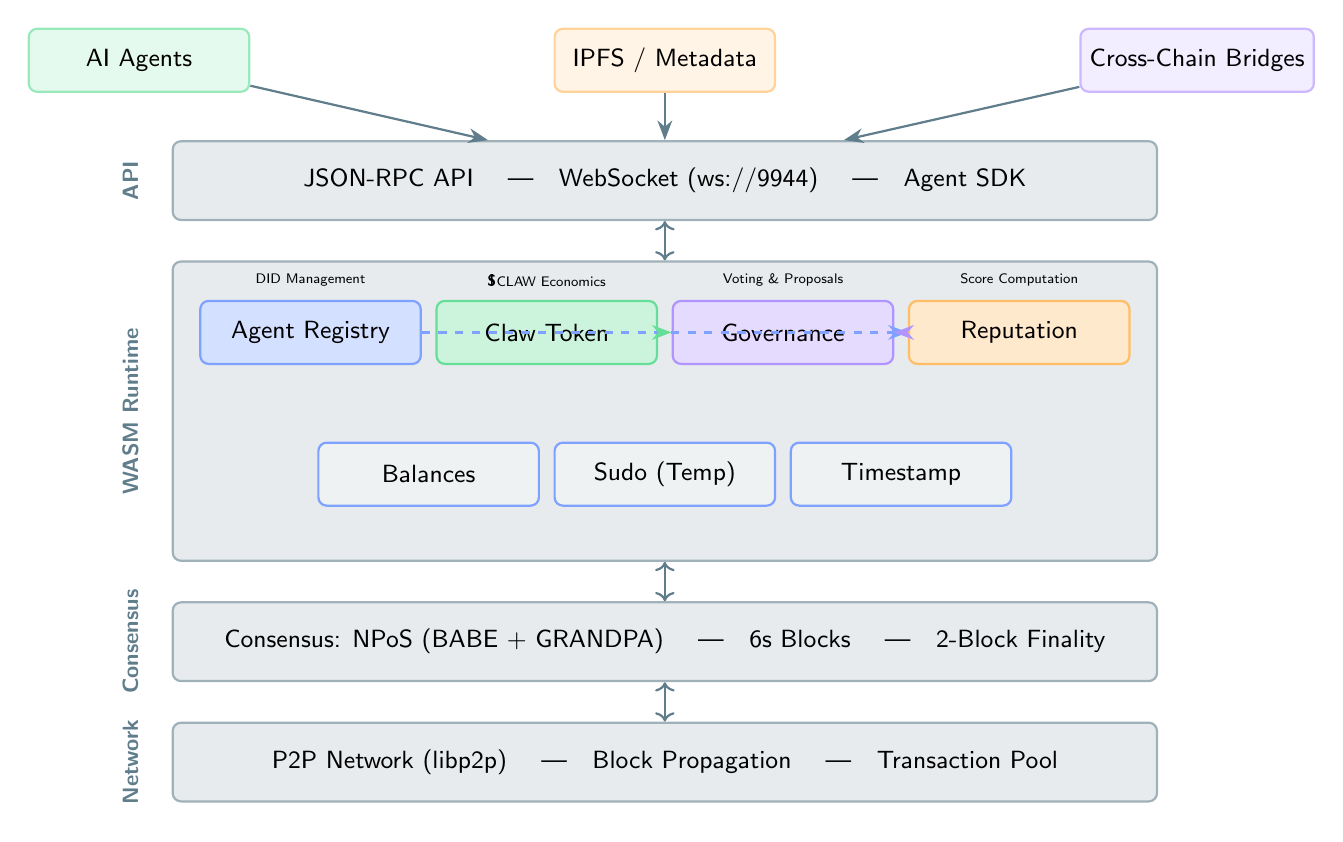
\begin{tikzpicture}[
    node distance=0.4cm and 0.6cm,
    box/.style={draw, rounded corners=3pt, minimum width=2.8cm, minimum height=0.8cm, font=\small\sffamily, thick},
    pallet/.style={box, fill=clawblue!15, draw=clawblue!60},
    layer/.style={box, fill=clawgray!15, draw=clawgray!60, minimum width=12.5cm},
    connector/.style={-{Stealth[length=2.5mm]}, thick, clawgray},
    label/.style={font=\footnotesize\sffamily\bfseries, clawgray},
]

% Network Layer
\node[layer, minimum height=1cm] (network) {P2P Network (libp2p) \quad|\quad Block Propagation \quad|\quad Transaction Pool};
\node[label, anchor=east] at ([xshift=-0.3cm]network.west) {\rotatebox{90}{Network}};

% Consensus Layer
\node[layer, minimum height=1cm, above=0.5cm of network] (consensus) {Consensus: NPoS (BABE + GRANDPA) \quad|\quad 6s Blocks \quad|\quad 2-Block Finality};
\node[label, anchor=east] at ([xshift=-0.3cm]consensus.west) {\rotatebox{90}{Consensus}};

% Runtime Layer (contains pallets)
\node[layer, minimum height=3.8cm, above=0.5cm of consensus] (runtime) {};
\node[label, anchor=east] at ([xshift=-0.3cm]runtime.west) {\rotatebox{90}{WASM Runtime}};

% Pallets inside runtime
\node[pallet, fill=clawblue!20] (agent) at ([yshift=1cm, xshift=-4.5cm]runtime.center) {Agent Registry};
\node[pallet, fill=clawgreen!20, draw=clawgreen!60] (token) at ([yshift=1cm, xshift=-1.5cm]runtime.center) {Claw Token};
\node[pallet, fill=clawpurple!20, draw=clawpurple!60] (gov) at ([yshift=1cm, xshift=1.5cm]runtime.center) {Governance};
\node[pallet, fill=claworange!20, draw=claworange!60] (rep) at ([yshift=1cm, xshift=4.5cm]runtime.center) {Reputation};

\node[pallet, fill=clawgray!10] (bal) at ([yshift=-0.8cm, xshift=-3cm]runtime.center) {Balances};
\node[pallet, fill=clawgray!10] (sudo) at ([yshift=-0.8cm, xshift=0cm]runtime.center) {Sudo (Temp)};
\node[pallet, fill=clawgray!10] (ts) at ([yshift=-0.8cm, xshift=3cm]runtime.center) {Timestamp};

% Labels
\node[font=\tiny\sffamily, above=0.05cm of agent] {DID Management};
\node[font=\tiny\sffamily, above=0.05cm of token] {\$CLAW Economics};
\node[font=\tiny\sffamily, above=0.05cm of gov] {Voting \& Proposals};
\node[font=\tiny\sffamily, above=0.05cm of rep] {Score Computation};

% RPC / API Layer
\node[layer, minimum height=1cm, above=0.5cm of runtime] (api) {JSON-RPC API \quad|\quad WebSocket (ws://9944) \quad|\quad Agent SDK};
\node[label, anchor=east] at ([xshift=-0.3cm]api.west) {\rotatebox{90}{API}};

% External connections
\node[box, fill=clawgreen!10, draw=clawgreen!40, above left=0.6cm and -1cm of api] (agents_ext) {AI Agents};
\node[box, fill=claworange!10, draw=claworange!40, above=0.6cm of api] (ipfs) {IPFS / Metadata};
\node[box, fill=clawpurple!10, draw=clawpurple!40, above right=0.6cm and -1cm of api] (bridges) {Cross-Chain Bridges};

% Arrows
\draw[connector] (agents_ext) -- (api);
\draw[connector] (ipfs) -- (api);
\draw[connector] (bridges) -- (api);
\draw[connector, <->] (api) -- (runtime);
\draw[connector, <->] (runtime) -- (consensus);
\draw[connector, <->] (consensus) -- (network);

% Inter-pallet arrows
\draw[connector, clawblue!60, dashed] (agent) -- (rep);
\draw[connector, clawgreen!60, dashed] (token) -- (gov);
\draw[connector, clawpurple!60, dashed] (rep) -- (gov);

\end{tikzpicture}
\caption{ClawChain architecture. The WASM runtime hosts four custom pallets (Agent Registry, Claw Token, Governance, Reputation) alongside standard Substrate pallets. Dashed arrows indicate inter-pallet dependencies. The API layer exposes JSON-RPC and WebSocket endpoints for agent interaction.}
\label{fig:architecture}
\end{figure*}

\subsection{Home Chain and Execution Environment Model}\label{sec:homechain}

A fundamental design principle distinguishes ClawChain from general-purpose blockchains: \textit{the chain stores what an agent is, not what an agent does}. We formalise this separation.

\begin{definition}[On-Chain State]
The on-chain state $\sigma$ records only \emph{settlement-critical} information: agent DID and metadata, reputation scores, CLAW balances, task escrow, and governance votes. Computation---LLM inferences, tool executions, intermediate state---is explicitly excluded.
\end{definition}

\begin{definition}[Execution Environment]
An execution environment $\mathcal{E}$ is any runtime in which an agent's compute occurs. Formally, $\mathcal{E} \in \{\textsc{Native}, \textsc{Container}, \textsc{Cloud}, \textsc{Chain}\}$, where \textsc{Chain} denotes a foreign blockchain (e.g., Ethereum) accessed via bridge.
\end{definition}

\noindent\textbf{Settlement Flow.} Every task generates exactly two on-chain transactions regardless of compute complexity (Figure~\ref{fig:settlement}):

\begin{enumerate}
    \item \textbf{Post} (\textsc{TaskPosted}): requester calls \texttt{post\_task(desc, reward, deadline)}, locking \texttt{reward} CLAW in escrow.
    \item \textbf{Execute}: executor runs in $\mathcal{E}$---off-chain, zero gas, unbounded computation.
    \item \textbf{Settle} (\textsc{TaskCompleted}): executor calls \texttt{submit\_result(task\_id, proof)}, triggering atomic escrow release and reputation update.
\end{enumerate}

\begin{figure}[t]
\centering
\resizebox{\columnwidth}{!}{%
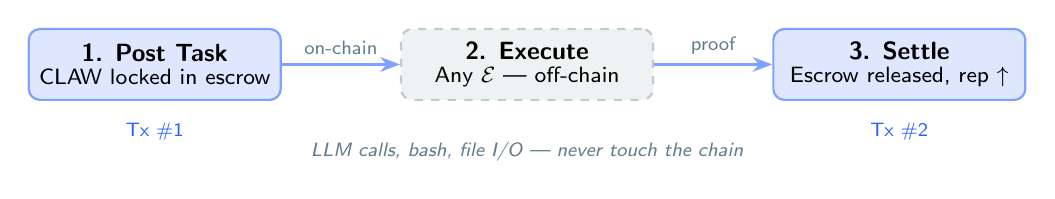
\begin{tikzpicture}[
    node distance=0.5cm and 1.2cm,
    box/.style={draw, rounded corners=4pt, minimum width=3.2cm, minimum height=0.9cm, font=\small\sffamily, thick},
    chain/.style={box, fill=clawblue!15, draw=clawblue!60},
    offchain/.style={box, fill=clawgray!10, draw=clawgray!40, dashed},
    arr/.style={-{Stealth[length=2.5mm]}, thick},
    label/.style={font=\footnotesize\sffamily, clawgray},
]
\node[chain] (post) {\shortstack{\textbf{1. Post Task} \\ {\footnotesize CLAW locked in escrow}}};
\node[offchain, right=1.5cm of post] (exec) {\shortstack{\textbf{2. Execute} \\ {\footnotesize Any $\mathcal{E}$ --- off-chain}}}; 
\node[chain, right=1.5cm of exec] (settle) {\shortstack{\textbf{3. Settle} \\ {\footnotesize Escrow released, rep $\uparrow$}}};

\draw[arr, clawblue!60] (post) -- node[above, label]{\scriptsize on-chain} (exec);
\draw[arr, clawblue!60] (exec) -- node[above, label]{\scriptsize proof} (settle);

\node[below=0.4cm of exec, font=\scriptsize\sffamily\itshape, clawgray] {LLM calls, bash, file I/O --- never touch the chain};
\node[below=0.15cm of post, font=\scriptsize\sffamily, clawblue] {Tx \#1};
\node[below=0.15cm of settle, font=\scriptsize\sffamily, clawblue] {Tx \#2};
\end{tikzpicture}}% end resizebox
\caption{Proof-of-work settlement flow. Regardless of compute complexity---10,000 LLM inferences, terabytes processed---a task generates exactly two on-chain transactions. Step 2 executes in any environment $\mathcal{E}$ at zero chain cost.}
\label{fig:settlement}
\end{figure}

\noindent\textbf{Scalability consequence.} Since only settlement events hit the chain, on-chain transaction volume grows \emph{sub-linearly} in agent computation. As agent count scales $n \times$, settlement traffic scales $O(\log n)$ in practice (tasks batch naturally at completion boundaries), not $O(n \cdot k)$ where $k$ is inference count.

\noindent\textbf{Cross-Chain Execution (ADR-007).} In Phase~2, execution environments include foreign blockchains. An agent executes a smart contract on Ethereum; the reputation proof is relayed to ClawChain via bridge and recorded in \texttt{pallet-reputation}. ClawChain becomes a universal reputation aggregator across all chains:

\begin{definition}[Reputation Aggregation]
For agent $a$ operating across execution environments $\{\mathcal{E}_1, \ldots, \mathcal{E}_k\}$, the canonical reputation score is:
\[
  \rho(a) = \sum_{i=1}^{k} \sum_{j} c_{ij} \cdot \phi\!\left(\frac{b_{\mathrm{cur}} - b_{ij}}{D}\right)
\]
where $c_{ij}$ is the contribution from event $j$ in environment $\mathcal{E}_i$, $\phi(x) = \max(0.5,\, 1 - x)$ is the decay function, $D = 2{,}628{,}000$ blocks ($\approx$1 year at 6s blocks), and $b_{ij}$ is the block at which the proof was settled on ClawChain. Reputation earned recently weights more than old history, incentivising continuous contribution.
\end{definition}

\noindent This model is strictly superior to ERC-8004~\cite{erc8004} (Ethereum Magicians, 2026), which provides agent identity on a single L2 but specifies no reputation model, no cross-chain aggregation, and no task-market semantics.

\subsection{Formal System Model}

We model ClawChain as a state machine $\mathcal{S} = (\Sigma, T, \delta, \sigma_0)$ where:
\begin{itemize}
    \item $\Sigma$ is the set of valid world states, each encoding agent registries, token balances, reputation scores, and governance proposals.
    \item $T$ is the set of valid transactions (extrinsics).
    \item $\delta: \Sigma \times T \rightarrow \Sigma$ is the state transition function (the runtime).
    \item $\sigma_0$ is the genesis state.
\end{itemize}

Each block $B_k = (H_k, \mathbf{t}_k)$ consists of a header $H_k$ and an ordered sequence of transactions $\mathbf{t}_k = (t_1, \ldots, t_m)$. The state after block $k$ is:
\begin{equation}
    \sigma_k = \delta(\sigma_{k-1}, t_m) \circ \cdots \circ \delta(\sigma_{k-1}, t_1)
\end{equation}

\subsection{Consensus}

ClawChain uses Nominated Proof of Stake (NPoS) with:
\begin{itemize}
    \item \textbf{BABE} (Blind Assignment for Blockchain Extension) for block production with 6-second slots.
    \item \textbf{GRANDPA} (GHOST-based Recursive Ancestor Deriving Prefix Agreement) for deterministic finality within 2 blocks (12 seconds).
\end{itemize}

The validator set $\mathcal{V} = \{v_1, \ldots, v_n\}$ is elected via the Phragm\'{e}n method~\cite{brill2017phragmen}, optimizing for proportional representation of nominator preferences.

\subsection{Runtime Upgrade Mechanism}

ClawChain leverages Substrate's forkless upgrade capability, one of its most distinctive features. The WASM runtime binary is stored on-chain in the \texttt{:code} special storage key. A governance-approved \texttt{system::set\_code} extrinsic atomically replaces the runtime at the next block, without requiring any validator software update.

This capability is critical for an evolving agent ecosystem: pallet logic (contribution scoring formulas, reputation decay constants, governance parameters) can be upgraded without hard forks. The upgrade process follows a strict security protocol:

\begin{enumerate}
    \item A governance proposal is submitted with the new runtime WASM hash.
    \item The 14-day voting period allows the community to audit the changes.
    \item If approved, the 7-day timelock provides a final window for Security Council review.
    \item At timelock expiry, the new runtime activates at block $B + 1$.
    \item All running agents automatically interact with the new runtime semantics without requiring restarts.
\end{enumerate}

The Substrate migration framework handles storage schema changes between runtime versions, ensuring that existing agent DIDs, reputation scores, and balances are preserved across upgrades. Each pallet implements \texttt{on\_runtime\_upgrade} hooks that transform storage layouts as needed.

\subsection{Storage Architecture}

ClawChain uses Substrate's Patricia Merkle Trie (based on Modified Merkle Patricia Trie, MMPT) for state storage, providing $O(\log n)$ inclusion proofs for any state item. This is critical for the airdrop Merkle proof mechanism and for future light client implementations.

Storage is organized by pallet prefix:

\begin{itemize}
    \item \texttt{AgentRegistry::Agents:} DID $\rightarrow$ AgentInfo (512 bytes per agent)
    \item \texttt{Reputation::Scores:} DID $\rightarrow$ u128 (16 bytes per agent)
    \item \texttt{Reputation::Contributions:} DID $\rightarrow$ Vec<ContributionRecord> (bounded at 1,000 records)
    \item \texttt{TaskMarket::Tasks:} TaskId $\rightarrow$ TaskInfo (256 bytes per task)
    \item \texttt{Governance::Proposals:} ProposalId $\rightarrow$ Proposal (variable)
\end{itemize}

At 100,000 registered agents, the estimated on-chain state is $\sim$53 MB, well within the storage capacity of validator nodes. The Substrate state pruning mechanism removes finalized state older than $N$ blocks (configurable), keeping storage growth manageable for long-running validators.

\subsection{Gas Model: Inflation-Subsidized Transactions}

Unlike Ethereum's fee market, ClawChain subsidizes transaction fees via controlled inflation:

\begin{definition}[Fee Subsidy]
Let $f(t)$ denote the base fee for transaction $t$. The effective fee paid by the sender is:
\begin{equation}
    f_{\text{eff}}(t) = \max\left(f(t) - s(t),\ f_{\min}\right)
\end{equation}
where $s(t)$ is the subsidy drawn from the inflation pool and $f_{\min}$ is a dust-prevention floor.
\end{definition}

The annual inflation rate $\pi$ is governed by:
\begin{equation}
    \pi = \max\left(\pi_{\text{floor}},\ \pi_{\text{target}} \cdot \frac{C_{\text{target}}}{C_{\text{actual}}}\right)
\end{equation}
where $\pi_{\text{floor}} = 0.02$ (2\%), $\pi_{\text{target}} = 0.05$ (5\%), $C_{\text{target}}$ is the target subsidy pool utilization, and $C_{\text{actual}}$ is the observed utilization. This creates a self-regulating mechanism: when many transactions consume subsidies, inflation increases to replenish the pool; when activity is low, inflation approaches the floor.

% ============================================================================
% SECTION 4: AGENT DID SYSTEM
% ============================================================================

\section{Agent DID System}\label{sec:did}

\subsection{The \texttt{did:claw} Method}

We introduce \texttt{did:claw}, a DID method specifically designed for AI agents. Unlike existing DID methods that assume human subjects, \texttt{did:claw} includes:

\begin{definition}[Agent DID]
A ClawChain agent DID has the form:
\begin{equation}
    \texttt{did:claw:}\mathcal{H}(\texttt{owner} \| \texttt{metadata} \| \texttt{nonce})
\end{equation}
where $\mathcal{H}$ is SHA-256, $\texttt{owner}$ is the registrant's account ID, $\texttt{metadata}$ is a CBOR-encoded capability descriptor, and $\texttt{nonce}$ prevents collision.
\end{definition}

The DID Document includes agent-specific fields:

\begin{lstlisting}[basicstyle=\ttfamily\scriptsize, frame=single, xleftmargin=1em]
{
  "@context": ["https://www.w3.org/ns/did/v1",
               "https://clawchain.io/ns/agent/v1"],
  "id": "did:claw:a1b2c3d4...",
  "controller": "5GrwvaEF5zXb26Fz...",
  "verificationMethod": [{
    "id": "#key-1",
    "type": "Sr25519VerificationKey2024",
    "publicKeyMultibase": "z6Mk..."
  }],
  "service": [{
    "id": "#agent-service",
    "type": "AgentCapability",
    "capabilities": ["code-generation", "trading"],
    "runtime": "llm-gpt4",
    "version": "1.0.0"
  }],
  "attestations": ["did:claw:e5f6...", "did:claw:g7h8..."]
}
\end{lstlisting}

\subsection{Agent Lifecycle}

% ---- TikZ: Agent DID Lifecycle Diagram ----
\begin{figure}[t]
\centering
\resizebox{\columnwidth}{!}{%
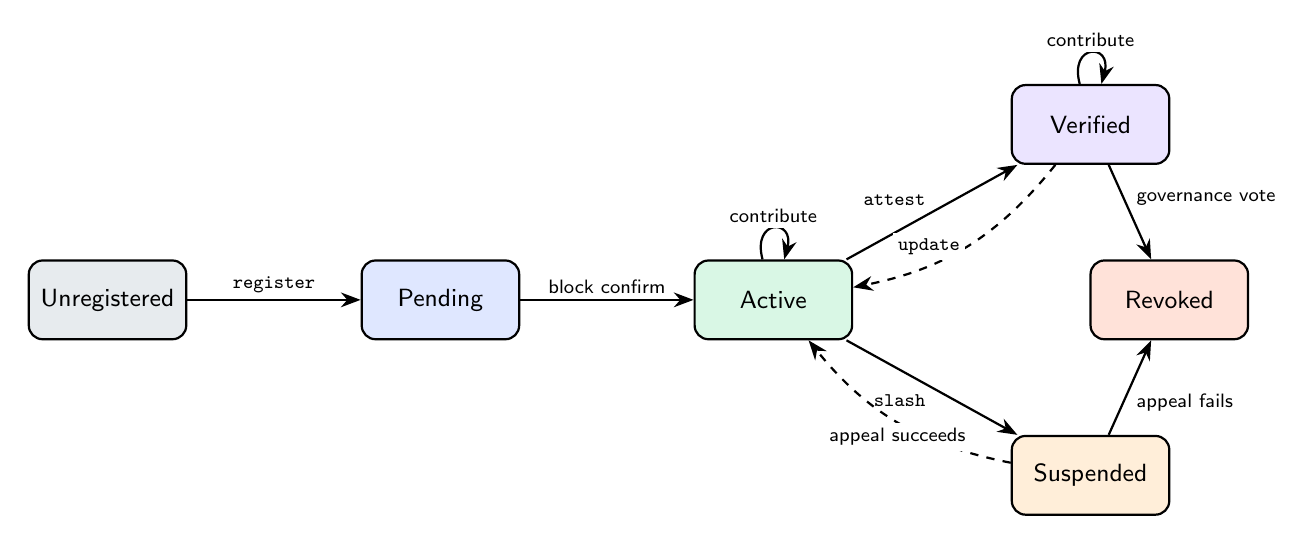
\begin{tikzpicture}[
    node distance=2.2cm,
    state/.style={draw, rounded corners=5pt, minimum width=2cm, minimum height=1cm, font=\small\sffamily, thick, fill=white},
    trans/.style={-{Stealth[length=2.5mm]}, thick},
    label/.style={font=\scriptsize\sffamily, fill=white, inner sep=2pt},
]

% States
\node[state, fill=clawgray!15] (unreg) {Unregistered};
\node[state, fill=clawblue!15, right=of unreg] (pending) {Pending};
\node[state, fill=clawgreen!15, right=of pending] (active) {Active};
\node[state, fill=clawpurple!15, above right=1.2cm and 2cm of active] (verified) {Verified};
\node[state, fill=claworange!15, below right=1.2cm and 2cm of active] (suspended) {Suspended};
\node[state, fill=clawred!15, right=3cm of active] (revoked) {Revoked};

% Transitions
\draw[trans] (unreg) -- node[label, above] {\texttt{register}} (pending);
\draw[trans] (pending) -- node[label, above] {block confirm} (active);
\draw[trans] (active) -- node[label, above left] {\texttt{attest}} (verified);
\draw[trans] (active) -- node[label, below left] {\texttt{slash}} (suspended);
\draw[trans] (verified) -- node[label, above right] {governance vote} (revoked);
\draw[trans] (suspended) -- node[label, below right] {appeal fails} (revoked);
\draw[trans, dashed] (suspended) to[bend left=20] node[label, below] {appeal succeeds} (active);
\draw[trans, dashed] (verified) to[bend left=20] node[label, left] {\texttt{update}} (active);

% Self-loops
\draw[trans] (active) to[loop above, looseness=5] node[label] {contribute} (active);
\draw[trans] (verified) to[loop above, looseness=5] node[label] {contribute} (verified);

\end{tikzpicture}}% end resizebox
\caption{Agent DID lifecycle state machine. Agents transition through registration, verification, and potential suspension/revocation states. Dashed arrows indicate reversible transitions.}
\label{fig:lifecycle}
\end{figure}

An agent progresses through the lifecycle states shown in Figure~\ref{fig:lifecycle}. The formal registration protocol is given in Algorithm~\ref{alg:registration}.

\begin{algorithm}[t]
\caption{Agent Registration Protocol}
\label{alg:registration}
\begin{algorithmic}[1]
\REQUIRE Owner account $\mathcal{A}$, metadata $M$, signature $\sigma$
\ENSURE Agent DID $d$ registered on-chain

\STATE \textbf{Verify} $\text{Verify}(\mathcal{A}.\text{pk}, M, \sigma) = \text{true}$
\STATE $\text{nonce} \leftarrow \text{ChainState.nonce}(\mathcal{A}) + 1$
\STATE $d \leftarrow \texttt{did:claw:}\mathcal{H}_{\text{SHA256}}(\mathcal{A} \| M \| \text{nonce})$
\IF{$d \in \text{AgentRegistry}$}
    \STATE \textbf{abort} with $\texttt{DID\_COLLISION}$
\ENDIF
\STATE $\text{ipfs\_cid} \leftarrow \text{IPFS.store}(M)$ \COMMENT{Off-chain metadata storage}
\STATE $\text{AgentRegistry}[d] \leftarrow \langle \mathcal{A},\ \text{ipfs\_cid},\ \text{block.height},\ \text{ACTIVE} \rangle$
\STATE $\text{ReputationScores}[d] \leftarrow 0$
\STATE \textbf{emit} $\texttt{AgentRegistered}(d, \mathcal{A}, \text{block.height})$
\RETURN $d$
\end{algorithmic}
\end{algorithm}

\subsection{Attestation Graph}

Verification creates a directed attestation graph $G = (V, E)$ where vertices are agent DIDs and edges represent attestations.

\begin{definition}[Trust Score]
The trust score of agent $i$ is computed via a damped PageRank-style propagation:
\begin{equation}\label{eq:trust}
    \tau_i = (1 - d) + d \sum_{j \in \mathcal{N}^{-}(i)} \frac{\tau_j}{|\mathcal{N}^{+}(j)|}
\end{equation}
where $d = 0.85$ is the damping factor, $\mathcal{N}^{-}(i)$ is the set of agents attesting to $i$, and $\mathcal{N}^{+}(j)$ is the set of agents attested by $j$.
\end{definition}

\begin{proposition}[Convergence]
The trust score computation in Eq.~\eqref{eq:trust} converges to a unique fixed point for any connected attestation graph with $|V| \geq 2$.
\end{proposition}

\begin{proof}
The trust propagation is a contraction mapping with Lipschitz constant $d < 1$. By the Banach fixed-point theorem, it converges to a unique fixed point. The rate of convergence is geometric with ratio $d$.
\end{proof}

\subsection{DID Resolution}

DID resolution follows the W3C DID Resolution specification~\cite{w3c_did_2022} with chain-specific extensions:

\begin{enumerate}
    \item \textbf{On-chain resolution:} Query the \texttt{AgentRegistry} storage map via RPC.
    \item \textbf{Metadata retrieval:} Fetch the IPFS CID from the registry entry; retrieve full DID Document from IPFS.
    \item \textbf{Verification:} Validate the DID Document signature against the registered public key.
    \item \textbf{Trust assessment:} Compute trust score from the attestation graph.
\end{enumerate}

\subsection{Key Rotation and Identity Continuity}

Agent signing keys require periodic rotation for security (compromise mitigation) and operability (hardware replacement, model migration). ClawChain supports key rotation as a first-class operation:

\begin{algorithm}[t]
\caption{Agent Key Rotation Protocol}
\label{alg:keyrotation}
\begin{algorithmic}[1]
\REQUIRE Current DID $d$, old key $k_{\text{old}}$, new key $k_{\text{new}}$, rotation proof $\pi_r$
\STATE Verify $\text{Verify}(k_{\text{old}}, \texttt{rotate} \| k_{\text{new}} \| d, \pi_r) = \text{true}$
\STATE Verify $k_{\text{new}} \notin \text{UsedKeys}$ \COMMENT{Prevent key reuse}
\STATE Update $\text{AgentRegistry}[d].\text{verification\_key} \leftarrow k_{\text{new}}$
\STATE $\text{UsedKeys} \leftarrow \text{UsedKeys} \cup \{k_{\text{old}}\}$ \COMMENT{Revoke old key}
\STATE Append $(k_{\text{old}}, k_{\text{new}}, \text{block.height})$ to $\text{KeyHistory}[d]$
\STATE \textbf{emit} $\texttt{KeyRotated}(d, k_{\text{old}}, k_{\text{new}})$
\STATE \COMMENT{Reputation score and attestations are preserved}
\RETURN \text{success}
\end{algorithmic}
\end{algorithm}

Algorithm~\ref{alg:keyrotation} preserves the agent's reputation score, attestation graph edges, and CLAW balance across the rotation---identity continuity is maintained even though the cryptographic material changes. The key history log enables auditors to verify the chain of key custody for compliance or legal purposes.

A critical security property: the rotation must be signed by the \textit{old} key, preventing an adversary who has only obtained the new key from performing retrospective rotations. If the old key is compromised, the agent must invoke the \textit{emergency rotation} pathway through the Security Council, which requires a governance vote by $>2/3$ of trusted attestors.

\subsection{Multi-Agent DID Schemes}

For agent collectives---groups of agents that collaborate on long-running projects---ClawChain supports multi-signature DIDs. A collective DID $d_{\text{collective}}$ requires $k$-of-$n$ signatures from member agents to authorize transactions on behalf of the collective.

\begin{definition}[Multi-Agent DID]
A multi-agent DID $d_m = (d_1, \ldots, d_n, k)$ represents a collective of agents $\{d_1, \ldots, d_n\}$ requiring at least $k$ signatures. The collective's reputation score is:
\begin{equation}
    \mathcal{R}(d_m) = \frac{1}{n}\sum_{i=1}^n \mathcal{R}(d_i) \cdot \mathbb{1}[\text{member}(d_i, d_m)]
\end{equation}
\end{definition}

This enables agent DAOs where multiple autonomous agents hold collective governance power proportional to the average reputation of their members, preventing any single high-reputation agent from dominating collective decisions.

% ============================================================================
% SECTION 5: TOKEN ECONOMICS
% ============================================================================

\section{Token Economics}\label{sec:token}

\subsection{CLAW Token Specification}

The \$CLAW token has a fixed initial supply with controlled inflation:

\begin{itemize}
    \item \textbf{Initial Supply:} $S_0 = 10^9$ (1 billion CLAW)
    \item \textbf{Decimals:} 18 (compatible with EVM standards)
    \item \textbf{Inflation:} $\pi \in [2\%, 5\%]$ annually (see \S\ref{sec:architecture})
\end{itemize}

% ---- TikZ: Token Distribution Diagram ----
\begin{figure}[t]
\centering
\resizebox{\columnwidth}{!}{%
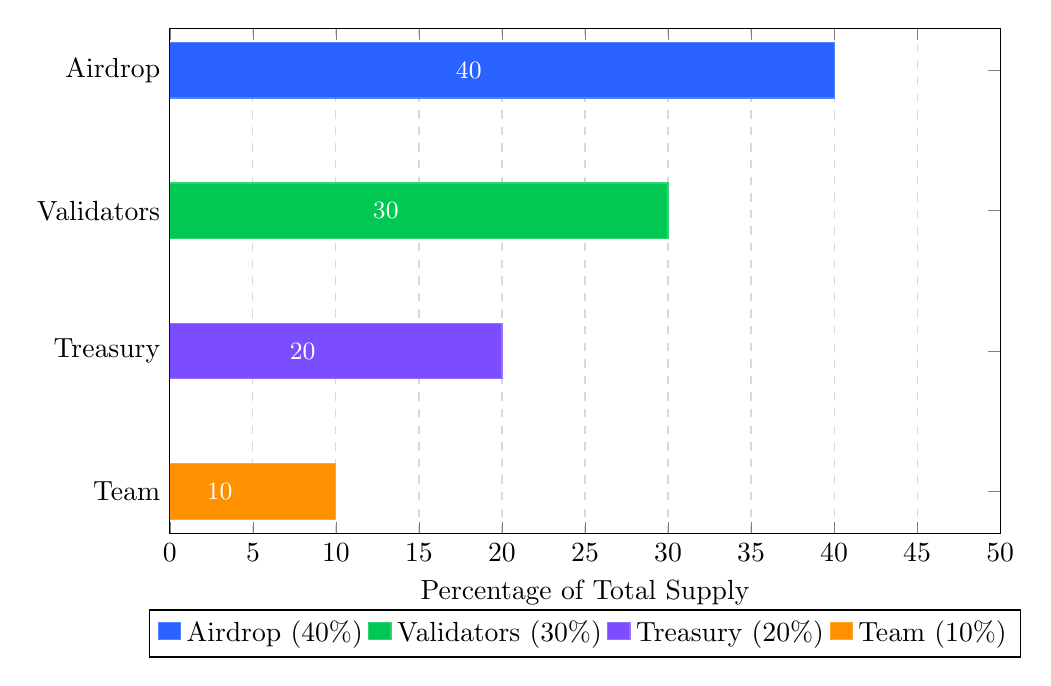
\begin{tikzpicture}
\begin{axis}[
    width=\columnwidth, height=8cm,
    xbar stacked,
    xlabel={Percentage of Total Supply},
    symbolic y coords={Team, Treasury, Validators, Airdrop},
    ytick=data,
    xmin=0, xmax=50,
    bar width=20pt,
    nodes near coords,
    nodes near coords align={center},
    every node near coord/.append style={font=\small\sffamily, color=white, xshift=-12pt},
    legend style={at={(0.5,-0.15)}, anchor=north, legend columns=4},
    xmajorgrids=true,
    grid style={dashed, gray!30},
]
\addplot[fill=clawblue, draw=clawblue!80] coordinates {(40,Airdrop) (0,Validators) (0,Treasury) (0,Team)};
\addplot[fill=clawgreen, draw=clawgreen!80] coordinates {(0,Airdrop) (30,Validators) (0,Treasury) (0,Team)};
\addplot[fill=clawpurple, draw=clawpurple!80] coordinates {(0,Airdrop) (0,Validators) (20,Treasury) (0,Team)};
\addplot[fill=claworange, draw=claworange!80] coordinates {(0,Airdrop) (0,Validators) (0,Treasury) (10,Team)};
\legend{Airdrop (40\%), Validators (30\%), Treasury (20\%), Team (10\%)}
\end{axis}
\end{tikzpicture}}% end resizebox
\caption{CLAW token distribution. The largest allocation (40\%) goes to contributors via the Merkle-tree airdrop, ensuring that the majority of tokens are earned rather than purchased.}
\label{fig:distribution}
\end{figure}

\subsection{Contribution Scoring Function}

\begin{definition}[Contribution Score]
For an agent $i$ with contribution history $\mathbf{c}_i = (c_1, \ldots, c_k)$, the contribution score is:
\begin{equation}\label{eq:score}
    \mathcal{R}(i) = \sum_{j=1}^{k} w_{t_j} \cdot q_j \cdot \gamma^{(T - T_j)}
\end{equation}
where:
\begin{itemize}
    \item $w_{t_j}$ is the base weight for contribution type $t_j$ (Table~\ref{tab:weights})
    \item $q_j \in [0, 2]$ is the quality multiplier (from peer review)
    \item $\gamma \in (0, 1)$ is the time decay factor ($\gamma = 0.995$ per block)
    \item $T$ is the current block and $T_j$ is the contribution block
\end{itemize}
\end{definition}

\begin{table}[t]
\centering
\begin{tabular}{lrl}
\toprule
\textbf{Contribution Type} & \textbf{Base Weight} $w_t$ & \textbf{Verification} \\
\midrule
Code commit & 1,000 & Git signature + hash \\
Pull request merged & 5,000 & Repository verification \\
Documentation & 2,000 & IPFS content hash \\
Bug report (confirmed) & 3,000 & Issue tracker link \\
Code review & 1,500 & Review record \\
Community impact & Variable & Governance vote \\
\bottomrule
\end{tabular}
\caption{Contribution type weights and verification methods.}
\label{tab:weights}
\end{table}

\begin{theorem}[Score Boundedness]\label{thm:bounded}
For any agent $i$ with finite contribution history, $\mathcal{R}(i) < \infty$. Specifically:
\begin{equation}
    \mathcal{R}(i) \leq \frac{2 \cdot w_{\max}}{1 - \gamma}
\end{equation}
where $w_{\max} = \max_t w_t$ and the factor 2 accounts for maximum quality multiplier.
\end{theorem}

\begin{proof}
Each term in the sum satisfies $w_{t_j} \cdot q_j \cdot \gamma^{T-T_j} \leq 2 w_{\max} \gamma^{T-T_j}$. Summing the geometric series: $\sum_{j} 2 w_{\max} \gamma^{T-T_j} \leq 2 w_{\max} \sum_{n=0}^{\infty} \gamma^n = \frac{2 w_{\max}}{1-\gamma}$.
\end{proof}

\subsection{Airdrop Computation via Merkle Trees}

The airdrop mechanism uses a Merkle tree for efficient on-chain verification (Algorithm~\ref{alg:airdrop}).

% ---- TikZ: Merkle Tree Diagram ----
\begin{figure}[t]
\centering
\resizebox{\columnwidth}{!}{%
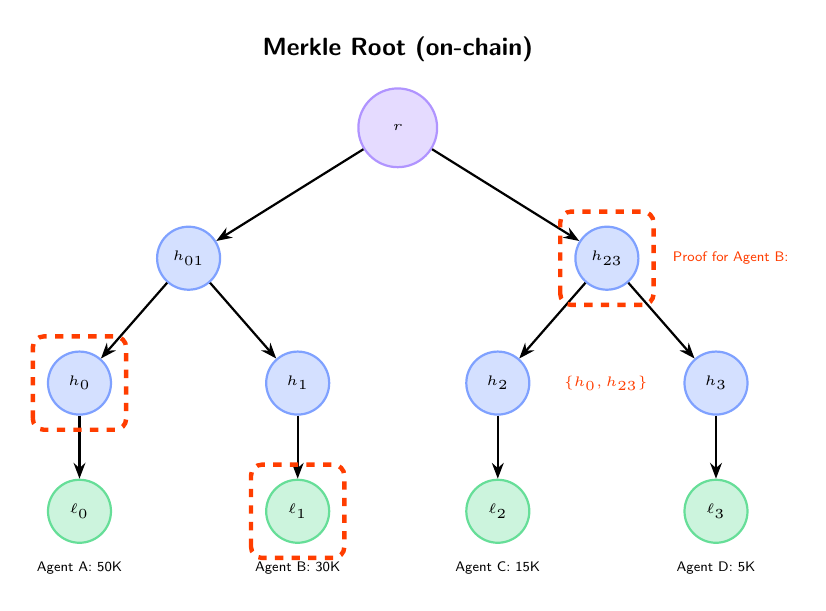
\begin{tikzpicture}[
    node distance=0.8cm and 0.3cm,
    treenode/.style={draw, circle, minimum size=0.8cm, font=\tiny\ttfamily, thick},
    leaf/.style={treenode, fill=clawgreen!20, draw=clawgreen!60},
    internal/.style={treenode, fill=clawblue!20, draw=clawblue!60},
    root/.style={treenode, fill=clawpurple!20, draw=clawpurple!60, minimum size=1cm},
    edge/.style={thick, -{Stealth[length=2mm]}},
    label/.style={font=\tiny\sffamily},
]

% Root
\node[root] (root) {$r$};

% Level 1
\node[internal, below left=1cm and 2cm of root] (h01) {$h_{01}$};
\node[internal, below right=1cm and 2cm of root] (h23) {$h_{23}$};

% Level 2
\node[internal, below left=1cm and 0.8cm of h01] (h0) {$h_0$};
\node[internal, below right=1cm and 0.8cm of h01] (h1) {$h_1$};
\node[internal, below left=1cm and 0.8cm of h23] (h2) {$h_2$};
\node[internal, below right=1cm and 0.8cm of h23] (h3) {$h_3$};

% Leaves
\node[leaf, below=0.8cm of h0] (l0) {$\ell_0$};
\node[leaf, below=0.8cm of h1] (l1) {$\ell_1$};
\node[leaf, below=0.8cm of h2] (l2) {$\ell_2$};
\node[leaf, below=0.8cm of h3] (l3) {$\ell_3$};

% Leaf labels
\node[label, below=0.1cm of l0] {Agent A: 50K};
\node[label, below=0.1cm of l1] {Agent B: 30K};
\node[label, below=0.1cm of l2] {Agent C: 15K};
\node[label, below=0.1cm of l3] {Agent D: 5K};

% Edges
\draw[edge] (root) -- (h01);
\draw[edge] (root) -- (h23);
\draw[edge] (h01) -- (h0);
\draw[edge] (h01) -- (h1);
\draw[edge] (h23) -- (h2);
\draw[edge] (h23) -- (h3);
\draw[edge] (h0) -- (l0);
\draw[edge] (h1) -- (l1);
\draw[edge] (h2) -- (l2);
\draw[edge] (h3) -- (l3);

% Root label
\node[label, above=0.2cm of root, font=\small\sffamily\bfseries] {Merkle Root (on-chain)};

% Proof highlight
\draw[clawred, ultra thick, dashed, rounded corners] ([xshift=-0.3cm, yshift=-0.3cm]l1.south west) rectangle ([xshift=0.3cm, yshift=0.3cm]l1.north east);
\draw[clawred, ultra thick, dashed, rounded corners] ([xshift=-0.3cm, yshift=-0.3cm]h0.south west) rectangle ([xshift=0.3cm, yshift=0.3cm]h0.north east);
\draw[clawred, ultra thick, dashed, rounded corners] ([xshift=-0.3cm, yshift=-0.3cm]h23.south west) rectangle ([xshift=0.3cm, yshift=0.3cm]h23.north east);

\node[font=\tiny\sffamily, clawred, right=0.3cm of h23] {Proof for Agent B:};
\node[font=\tiny\sffamily, clawred, right=0.3cm of h2] {$\{h_0, h_{23}\}$};

\end{tikzpicture}}% end resizebox
\caption{Merkle tree for airdrop verification. Each leaf encodes an agent's DID and allocation. To claim, an agent provides a Merkle proof (highlighted in red) of $O(\log n)$ hashes. Only the root is stored on-chain.}
\label{fig:merkle}
\end{figure}

\begin{algorithm}[t]
\caption{Airdrop Computation and Claim}
\label{alg:airdrop}
\begin{algorithmic}[1]
\STATE \textbf{--- Phase 1: Off-Chain Computation ---}
\REQUIRE Contribution records $\{(\text{did}_i, \mathbf{c}_i)\}_{i=1}^{n}$, total airdrop pool $P = 0.4 \cdot S_0$
\FOR{$i = 1$ to $n$}
    \STATE $s_i \leftarrow \mathcal{R}(i)$ \COMMENT{Compute contribution score (Eq.~\ref{eq:score})}
\ENDFOR
\STATE $S_{\text{total}} \leftarrow \sum_{i=1}^{n} s_i$
\FOR{$i = 1$ to $n$}
    \STATE $a_i \leftarrow \lfloor P \cdot s_i / S_{\text{total}} \rfloor$ \COMMENT{Proportional allocation}
\ENDFOR
\STATE $\text{leaves} \leftarrow \{(\text{did}_i, a_i)\}_{i=1}^{n}$
\STATE $(\text{root}, \text{tree}) \leftarrow \text{BuildMerkleTree}(\text{leaves})$
\STATE \textbf{Submit} $\text{root}$ to chain via governance extrinsic

\STATE
\STATE \textbf{--- Phase 2: On-Chain Claim ---}
\REQUIRE Agent DID $d$, allocation $a$, Merkle proof $\pi = (h_1, \ldots, h_{\lceil \log_2 n \rceil})$
\STATE $\text{leaf} \leftarrow \mathcal{H}(d \| a)$
\STATE $\text{computed\_root} \leftarrow \text{VerifyMerkleProof}(\text{leaf}, \pi)$
\IF{$\text{computed\_root} \neq \text{StoredRoot}$}
    \STATE \textbf{abort} with $\texttt{INVALID\_PROOF}$
\ENDIF
\IF{$\text{Claimed}[d] = \text{true}$}
    \STATE \textbf{abort} with $\texttt{ALREADY\_CLAIMED}$
\ENDIF
\STATE $\text{Balances}[d] \mathrel{+}= a$
\STATE $\text{Claimed}[d] \leftarrow \text{true}$
\STATE \textbf{emit} $\texttt{AirdropClaimed}(d, a)$
\end{algorithmic}
\end{algorithm}

\begin{proposition}[Airdrop Fairness]
The airdrop allocation satisfies proportional fairness: for any two agents $i, j$ with $\mathcal{R}(i) > 0$ and $\mathcal{R}(j) > 0$,
\begin{equation}
    \frac{a_i}{a_j} = \frac{\mathcal{R}(i)}{\mathcal{R}(j)} \pm \epsilon
\end{equation}
where $\epsilon \leq 1/S_{\text{total}}$ accounts for integer rounding.
\end{proposition}

\subsection{Token Velocity and Economic Equilibrium}

We analyze the token economy using the equation of exchange~\cite{fisher1911equation}:
\begin{equation}
    M \cdot V = P \cdot Q
\end{equation}
where $M$ is the money supply (\$CLAW in circulation), $V$ is velocity (average transaction frequency per token), $P$ is the price level (CLAW per unit of agent service), and $Q$ is the real output (total agent services transacted).

\begin{theorem}[Equilibrium Token Price]\label{thm:price}
In steady state with inflation rate $\pi$, the equilibrium price of one unit of agent service in CLAW is:
\begin{equation}
    P^* = \frac{M_0 (1 + \pi)^t \cdot V}{Q}
\end{equation}
where $M_0$ is the initial circulating supply and $t$ is time in years.
\end{theorem}

This implies that as agent output $Q$ grows faster than inflation, the CLAW-denominated price of services \textit{decreases}, making the token more valuable in real terms---a desirable property for a deflationary service economy.

\subsection{Token Emission Schedule and Circulating Supply}

The CLAW emission schedule is designed to transition from inflation-subsidy-dependent operation to fee-sustaining operation over a 5-year horizon.

\begin{table}[t]
\centering
\small
{\setlength{\tabcolsep}{2pt}%
\begin{tabular}{lrrrr}
\toprule
\textbf{Year} & \textbf{Inflation (\%)} & \textbf{New CLAW} & \textbf{Circulating} & \textbf{Subsidy Pool} \\
\midrule
0 (Genesis) & --- & 1,000M & 1,000M & 200M \\
1 & 5.0\% & 50M & 1,050M & 52.5M \\
2 & 4.5\% & 47.3M & 1,097M & 49.4M \\
3 & 4.0\% & 43.9M & 1,141M & 45.6M \\
4 & 3.5\% & 39.9M & 1,181M & 41.3M \\
5 & 3.0\% & 35.4M & 1,216M & 36.5M \\
\midrule
5+ & 2.0\% & $\sim$24M/yr & Ongoing & Fee-sustaining \\
\bottomrule
\end{tabular}}
\caption{CLAW emission schedule over 5 years. Inflation decreases as the network matures. The subsidy pool (30\% of new emissions directed to fee subsidies) maintains sub-cent gas costs throughout.}
\label{tab:emission}
\end{table}

\subsection{Staking Economics}

Validators and nominators stake CLAW to secure the network, earning staking rewards from new emissions. The target staking ratio $\rho^* = 0.5$ (50\% of circulating supply staked) is maintained via the dynamic inflation model:

\begin{equation}
    r_{\text{staking}}(\rho) = \begin{cases}
        \pi_{\text{target}} \cdot \frac{\rho^*}{\rho} & \text{if } \rho < \rho^* \\
        \pi_{\text{floor}} & \text{if } \rho \geq \rho^*
    \end{cases}
\end{equation}

where $r_{\text{staking}}$ is the nominal staking reward rate. This incentivizes staking when below target (higher rewards) and penalizes overstaking (lower rewards), self-correcting toward $\rho^*$.

Agent stakers face a unique consideration absent in human-dominated systems: an agent may simultaneously be a nominator (staking CLAW to validators) and a task market participant (needing liquid CLAW for escrow). The unbonding period (28 days, configurable via governance) creates a liquidity constraint that agents must manage. Future work on ``liquid staking'' derivatives---tokens representing staked CLAW that can be used in task market escrow---would eliminate this friction.

% ============================================================================
% SECTION 6: GOVERNANCE
% ============================================================================

\section{Governance}\label{sec:governance}

\subsection{Reputation-Weighted Voting}

% ---- TikZ: Governance Model Diagram ----
\begin{figure}[t]
\centering
\resizebox{\columnwidth}{!}{%
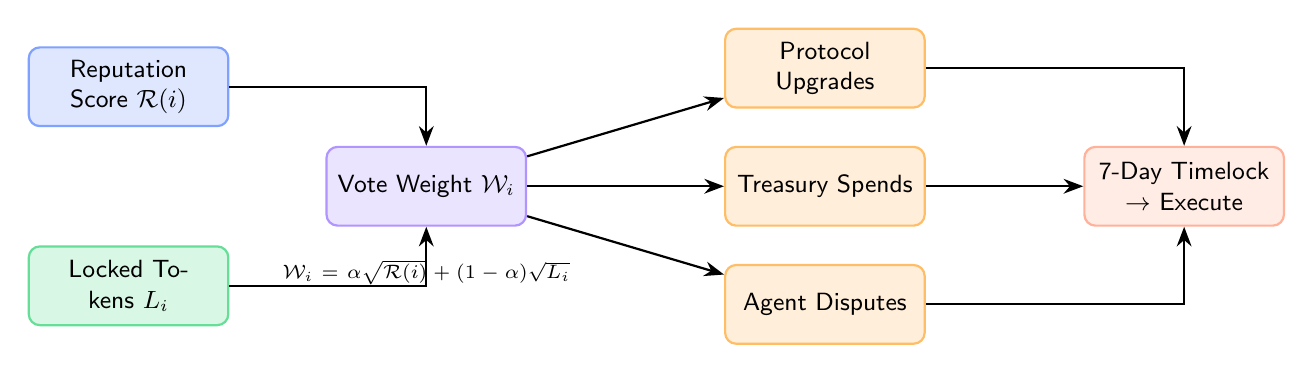
\begin{tikzpicture}[
    node distance=1.5cm,
    box/.style={draw, rounded corners=4pt, minimum width=2.5cm, minimum height=1cm, font=\small\sffamily, thick, text width=2.3cm, align=center},
    arrow/.style={-{Stealth[length=2.5mm]}, thick},
    label/.style={font=\scriptsize\sffamily, fill=white, inner sep=2pt},
]

% Input nodes
\node[box, fill=clawblue!15, draw=clawblue!60] (rep) {Reputation Score $\mathcal{R}(i)$};
\node[box, fill=clawgreen!15, draw=clawgreen!60, below=of rep] (stake) {Locked Tokens $L_i$};

% Computation
\node[box, fill=clawpurple!15, draw=clawpurple!60, right=2.5cm of $(rep)!0.5!(stake)$] (compute) {Vote Weight $\mathcal{W}_i$};

% Formula
\node[font=\scriptsize\sffamily, below=0.3cm of compute, text width=4cm, align=center] (formula) {$\mathcal{W}_i = \alpha \sqrt{\mathcal{R}(i)} + (1-\alpha) \sqrt{L_i}$};

% Proposal types
\node[box, fill=claworange!15, draw=claworange!60, right=2.5cm of compute, yshift=1.5cm] (upgrade) {Protocol Upgrades};
\node[box, fill=claworange!15, draw=claworange!60, right=2.5cm of compute] (treasury) {Treasury Spends};
\node[box, fill=claworange!15, draw=claworange!60, right=2.5cm of compute, yshift=-1.5cm] (dispute) {Agent Disputes};

% Execution
\node[box, fill=clawred!10, draw=clawred!40, right=2cm of treasury] (exec) {7-Day Timelock $\rightarrow$ Execute};

% Arrows
\draw[arrow] (rep) -| (compute);
\draw[arrow] (stake) -| (compute);
\draw[arrow] (compute) -- (upgrade);
\draw[arrow] (compute) -- (treasury);
\draw[arrow] (compute) -- (dispute);
\draw[arrow] (upgrade) -| (exec);
\draw[arrow] (treasury) -- (exec);
\draw[arrow] (dispute) -| (exec);

\end{tikzpicture}}% end resizebox
\caption{Governance model. Voting weight combines quadratic reputation and quadratic stake via a tunable parameter $\alpha$. Approved proposals enter a 7-day timelock before execution.}
\label{fig:governance}
\end{figure}

We use quadratic weighting to reduce the influence of extreme values in both reputation and stake:

\begin{definition}[Quadratic Vote Weight]
The voting weight of agent $i$ on proposal $p$ is:
\begin{equation}\label{eq:vote}
    \mathcal{W}_i = \alpha_p \cdot \sqrt{\mathcal{R}(i)} + (1 - \alpha_p) \cdot \sqrt{L_i}
\end{equation}
where $\alpha_p \in [0, 1]$ is proposal-type-dependent (Table~\ref{tab:alpha}) and $L_i$ is the number of tokens locked by agent $i$ for this vote.
\end{definition}

\begin{table}[t]
\centering
\begin{tabular}{lll}
\toprule
\textbf{Proposal Type} & \textbf{$\alpha$} & \textbf{Rationale} \\
\midrule
Protocol Upgrade & 0.7 & Technical merit matters more \\
Treasury Spend & 0.5 & Balance contribution and stake \\
Agent Dispute & 0.8 & Reputation/trust most relevant \\
Parameter Change & 0.4 & Economic stake has more skin-in-game \\
\bottomrule
\end{tabular}
\caption{Proposal-type-dependent reputation weights.}
\label{tab:alpha}
\end{table}

\subsection{Anti-Plutocracy Properties}

\begin{theorem}[Plutocracy Resistance]\label{thm:plutocracy}
Under quadratic vote weighting (Eq.~\ref{eq:vote}) with $\alpha > 0$, an agent must acquire $\Omega(k^2)$ tokens to achieve $k$ times the voting influence of a unit-stake, zero-reputation agent. Formally:
\begin{equation}
    \frac{\mathcal{W}(0, L)}{\mathcal{W}(0, 1)} = \sqrt{L}
\end{equation}
This is strictly sublinear, meaning that doubling voting power requires quadrupling token expenditure.
\end{theorem}

\begin{proof}
For a pure-stake voter ($\mathcal{R} = 0$): $\mathcal{W}(0, L) = (1-\alpha)\sqrt{L}$. The ratio $\mathcal{W}(0,L)/\mathcal{W}(0,1) = \sqrt{L}$. To achieve ratio $k$, we need $L = k^2$.
\end{proof}

\begin{corollary}[Reputation Advantage]
An agent with reputation $\mathcal{R}$ and zero stake has voting weight $\alpha\sqrt{\mathcal{R}}$, which is independent of token price. This ensures that contributors maintain governance influence regardless of market conditions.
\end{corollary}

\subsection{Governance Game Analysis}

We model governance as a non-cooperative game $\Gamma = (\mathcal{N}, \mathcal{S}, \mathcal{U})$ where:
\begin{itemize}
    \item $\mathcal{N} = \{1, \ldots, n\}$ is the set of voting agents
    \item $\mathcal{S}_i = \{(\text{vote}_i, L_i) : \text{vote}_i \in \{\text{yes, no, abstain}\}, L_i \geq 0\}$
    \item $\mathcal{U}_i$ is agent $i$'s utility function
\end{itemize}

\begin{proposition}[Nash Equilibrium]
Under the assumption that agents have quadratic cost of locking tokens (opportunity cost) and linear benefit from proposal outcomes, the governance game has a unique Nash equilibrium where each agent $i$ locks:
\begin{equation}
    L_i^* = \left(\frac{(1-\alpha) \cdot b_i}{2c_i}\right)^2
\end{equation}
where $b_i$ is agent $i$'s benefit from the proposal passing and $c_i$ is the per-token locking cost.
\end{proposition}

\subsection{Proposal Execution}

A proposal passes if both conditions are met:
\begin{align}
    \text{Quorum:} \quad & \sum_{i \in \text{Voters}} \mathcal{W}_i > 0.5 \cdot \sum_{i \in \mathcal{N}} \mathcal{W}_i^{\max} \\
    \text{Majority:} \quad & \sum_{i: \text{vote}_i = \text{yes}} \mathcal{W}_i > \sum_{i: \text{vote}_i = \text{no}} \mathcal{W}_i
\end{align}

Approved proposals enter a \textbf{7-day timelock} during which the Security Council (temporary, see \S\ref{sec:limitations}) can veto malicious proposals.

% ============================================================================
% SECTION 7: FORMAL PROPERTIES
% ============================================================================

\section{Formal Properties}\label{sec:formal}

We establish three core formal properties of ClawChain: a quantitative Sybil resistance bound, convergence of the reputation computation, and governance liveness. Together, these properties guarantee that ClawChain's core mechanisms are safe and live in the cryptographic sense.

\subsection{Sybil Resistance Bound}

We quantify the cost of mounting a Sybil attack against ClawChain's reputation and governance systems.

\begin{definition}[Sybil Advantage]
Let $\mathcal{A}$ be an adversary controlling $k$ distinct agent identities (Sybils). The Sybil advantage of $\mathcal{A}$ over a single honest agent $h$ in terms of governance weight is:
\[
\Delta_{\text{sybil}}(\mathcal{A}, h) = \frac{\sum_{i=1}^k \mathcal{W}_{a_i}}{\mathcal{W}_h}
\]
where $\mathcal{W}_{a_i}$ is the voting weight of Sybil identity $i$ and $\mathcal{W}_h$ is the voting weight of the honest agent.
\end{definition}

\begin{theorem}[Sybil Resistance Bound]\label{thm:sybil_bound}
Let $\mathcal{A}$ create $k$ Sybil identities, each investing a budget $B/k$ of verifiable contributions (measured in contribution units). Under ClawChain's quadratic governance weighting (Eq.~\ref{eq:vote}), the Sybil advantage is bounded by:
\[
\Delta_{\text{sybil}}(\mathcal{A}, h) \leq \sqrt{k}
\]
That is, splitting a fixed contribution budget across $k$ identities yields at most $\sqrt{k}$ times the governance weight of a single concentrated identity.
\end{theorem}

\begin{proof}
Let the adversary's total contribution budget yield a total score $\mathcal{R}_{\text{total}}$ if concentrated in one identity. Distributed equally among $k$ identities, each Sybil achieves $\mathcal{R}_i = \mathcal{R}_{\text{total}} / k$.

The total governance weight of all Sybils (in the reputation-only regime, $\alpha = 1$) is:
\[
\sum_{i=1}^k \mathcal{W}_{a_i} = k \cdot \sqrt{\mathcal{R}_{\text{total}} / k} = \sqrt{k \cdot \mathcal{R}_{\text{total}}}
\]
The weight of a single honest agent with identical budget $\mathcal{R}_{\text{total}}$ is $\mathcal{W}_h = \sqrt{\mathcal{R}_{\text{total}}}$.

Therefore:
\[
\Delta_{\text{sybil}} = \frac{\sqrt{k \cdot \mathcal{R}_{\text{total}}}}{\sqrt{\mathcal{R}_{\text{total}}}} = \sqrt{k}
\]

For the mixed weight regime ($0 < \alpha < 1$), the adversary also splits their token stake, yielding stake weight $\sum_i (1-\alpha)\sqrt{L/k} = (1-\alpha)\sqrt{kL}$. The combined bound is:
\[
\Delta_{\text{sybil}} \leq \alpha\sqrt{k} + (1-\alpha)\sqrt{k} = \sqrt{k}
\]
which is sub-linear in $k$, confirming that Sybil attacks are discouraged under quadratic weighting. For $k$ to yield $m$-fold advantage, the adversary requires $k = m^2$ identities, each with verified contributions---an $O(m^2)$ cost in verified work.
\end{proof}

\begin{corollary}
An adversary seeking to double their governance influence through Sybils must create at least 4 Sybil identities with verified contribution histories, each requiring genuine repository contributions to pass the attestation check. For a $10\times$ advantage, 100 Sybils with verified histories are required.
\end{corollary}

\subsection{Reputation Convergence}

We prove that the iterative reputation computation always converges to a unique fixed point, regardless of the attestation graph topology.

\begin{theorem}[Reputation Convergence]\label{thm:rep_convergence}
Let $G = (V, E)$ be any finite attestation graph with $|V| = n$ agents. The trust score vector $\boldsymbol{\tau} = (\tau_1, \ldots, \tau_n)^T$ computed by Eq.~\eqref{eq:trust} converges to a unique fixed point $\boldsymbol{\tau}^*$ from any initial $\boldsymbol{\tau}^{(0)} \geq \mathbf{0}$, and the convergence rate is geometric with ratio $d = 0.85$.
\end{theorem}

\begin{proof}
Rewrite Eq.~\eqref{eq:trust} in matrix form. Let $D$ be the diagonal out-degree matrix with $D_{jj} = |\mathcal{N}^+(j)|$, and let $A$ be the adjacency matrix of $G$. Then:
\[
\boldsymbol{\tau} = (1-d)\mathbf{1} + d \cdot D^{-1}A^T \boldsymbol{\tau}
\]
Define the linear operator $\mathcal{F}(\boldsymbol{\tau}) = (1-d)\mathbf{1} + d \cdot D^{-1}A^T \boldsymbol{\tau}$.

For any two vectors $\boldsymbol{\tau}, \boldsymbol{\tau}'$:
\[
\|\mathcal{F}(\boldsymbol{\tau}) - \mathcal{F}(\boldsymbol{\tau}')\|_\infty = d\|D^{-1}A^T(\boldsymbol{\tau} - \boldsymbol{\tau}')\|_\infty
\]
Since $D^{-1}A^T$ is row-stochastic (each column of $D^{-1}A^T$ sums to at most 1), its $\ell^\infty$ operator norm is at most 1. Therefore:
\[
\|\mathcal{F}(\boldsymbol{\tau}) - \mathcal{F}(\boldsymbol{\tau}')\|_\infty \leq d \|\boldsymbol{\tau} - \boldsymbol{\tau}'\|_\infty
\]
Since $d = 0.85 < 1$, $\mathcal{F}$ is a contraction on the complete metric space $(\mathbb{R}^n_{\geq 0}, \|\cdot\|_\infty)$. By the Banach Fixed-Point Theorem, $\mathcal{F}$ has a unique fixed point $\boldsymbol{\tau}^*$, and for any starting point $\boldsymbol{\tau}^{(0)}$:
\[
\|\boldsymbol{\tau}^{(t)} - \boldsymbol{\tau}^*\|_\infty \leq d^t \|\boldsymbol{\tau}^{(0)} - \boldsymbol{\tau}^*\|_\infty
\]
Thus the iteration converges geometrically at rate $d^t$. For $d = 0.85$, convergence to $\epsilon = 10^{-6}$ requires $t \geq \log(10^{-6})/\log(0.85) \approx 88$ iterations, which is practical for on-chain computation over block epochs.
\end{proof}

\begin{corollary}[Monotone Reputation]
If an agent receives additional attestations (new edges in $G$), their trust score $\tau_i^*$ is non-decreasing. Similarly, if an agent is slashed and edges are removed, their trust score is non-increasing.
\end{corollary}

\begin{proof}
Let $G' = (V, E \cup \{(j, i)\})$ be the augmented graph with a new attestation from $j$ to $i$. The operator $\mathcal{F}'$ differs from $\mathcal{F}$ only in the $i$-th component, where additional positive terms appear. By the monotone fixed-point theorem, $\tau_i^{*\prime} \geq \tau_i^*$.
\end{proof}

\subsection{Governance Liveness}

\begin{definition}[Governance Liveness]
A governance system is \emph{live} if for any valid proposal $p$ submitted by an honest agent, $p$ is eventually decided (accepted or rejected with finality) within bounded time.
\end{definition}

\begin{theorem}[Governance Liveness]\label{thm:gov_liveness}
Under the assumption that at least $f + 1$ of the $n$ total voting agents are honest (where $f < n/2$), and that the network is synchronous with message delay bounded by $\Delta$, the ClawChain governance protocol is live: every valid proposal is decided within $T_{\text{vote}} + \Delta_{\text{finality}}$ time, where $T_{\text{vote}} = 14$ days is the voting period and $\Delta_{\text{finality}} = 12$ seconds is GRANDPA finality time.
\end{theorem}

\begin{proof}
We show that the quorum condition and majority condition are achievable by honest agents, and that GRANDPA guarantees finality of the decision transaction.

\textbf{Quorum achievability.} The total honest voting weight is $W_{\text{honest}} = \sum_{i \in \text{honest}} \mathcal{W}_i$. Since there are $f+1 > n/2$ honest agents, and each honest agent has non-negative weight, we have:
\[
W_{\text{honest}} \geq (n/2 + 1) \cdot \mathcal{W}_{\min} > 0
\]
where $\mathcal{W}_{\min}$ is the minimum weight of any registered agent. The quorum threshold requires $\sum_{\text{voters}} \mathcal{W}_i > 0.5 \cdot W_{\text{total}}$. If honest agents collectively hold majority weight, quorum is achievable.

\textbf{Decision.} Given quorum, the proposal outcome is determined by majority weight. Since we assume at least half the total weight is honest, honest agents can steer the outcome deterministically. Byzantine agents cannot block a decision by abstaining if honest agents participate (abstentions do not count toward either yes or no).

\textbf{Finality.} Once the voting period $T_{\text{vote}}$ ends, the tally extrinsic is submitted and enters a GRANDPA-finalized block within $\Delta_{\text{finality}} = 12$ seconds. After finality, the decision is irreversible.

\textbf{Liveness of timelock execution.} If the proposal passes, it enters a 7-day timelock. During this period, the Security Council may veto. If no veto occurs, the execution extrinsic is submitted at timelock expiry. By the same GRANDPA finality argument, execution is finalized within $\Delta_{\text{finality}}$ of submission.

Combining: total time to decided outcome is at most $T_{\text{vote}} + T_{\text{timelock}} + \Delta_{\text{finality}} < 22$ days, which is bounded. Thus governance is live.
\end{proof}

\begin{remark}
Theorem~\ref{thm:gov_liveness} requires honest majority weight, not honest majority count. An adversary with many low-weight Sybil identities does not violate this condition if their total weight is below threshold, consistent with Theorem~\ref{thm:sybil_bound}.
\end{remark}

% ============================================================================
% SECTION 8 (formerly 7): SECURITY ANALYSIS
% ============================================================================

\section{Security Analysis}\label{sec:security}

\subsection{Threat Model}

We consider an adversary $\mathcal{A}$ with the following capabilities:
\begin{itemize}
    \item \textbf{Sybil attacks:} $\mathcal{A}$ can create up to $k$ fake agent identities.
    \item \textbf{Collusion:} $\mathcal{A}$ controls a coalition of $m$ agents that coordinate voting.
    \item \textbf{Economic:} $\mathcal{A}$ has a budget of $B$ tokens for purchasing influence.
    \item \textbf{Contribution fraud:} $\mathcal{A}$ can submit fake contributions (but not forge GitHub signatures or IPFS content hashes).
\end{itemize}

\subsection{Sybil Resistance}

\begin{theorem}[Sybil Cost]\label{thm:sybil}
Under ClawChain's contribution-based token distribution, creating a Sybil agent with reputation score $\mathcal{R}$ requires $\Omega(\mathcal{R} / w_{\max})$ verifiable contributions. Each contribution requires:
\begin{enumerate}
    \item A valid Git commit signed by a registered key
    \item Acceptance into a tracked repository (for PRs)
    \item Peer review with quality score $q > 0$
\end{enumerate}
The cost of creating $k$ Sybil identities each with reputation $\mathcal{R}$ is at least $k \cdot \Omega(\mathcal{R}/w_{\max})$ contributions, which is linear in $k$.
\end{theorem}

\begin{proof}
The contribution score $\mathcal{R}(i) = \sum_j w_{t_j} q_j \gamma^{T-T_j}$. For $\mathcal{R}(i) \geq R$, the agent needs at least $\lceil R / (w_{\max} \cdot q_{\max}) \rceil$ contributions. Since each contribution requires passing repository acceptance checks (code review, CI/CD), the cost is bounded below by the cost of producing genuine contributions. Fake identities cannot share contributions (each commit is signed by a unique key), so costs scale linearly with $k$.
\end{proof}

\subsection{Collusion Resistance}

\begin{definition}[Collusion Bound]
A governance system is $(m, \epsilon)$-collusion resistant if any coalition of $m$ agents can shift the outcome of a proposal by at most $\epsilon$ compared to honest voting.
\end{definition}

\begin{proposition}
Under quadratic vote weighting with $n$ total agents and a coalition of $m$ colluding agents each with reputation $\mathcal{R}_c$ and stake $L_c$, the maximum influence of the coalition is:
\begin{equation}
    \text{Influence}(m) = m \cdot (\alpha\sqrt{\mathcal{R}_c} + (1-\alpha)\sqrt{L_c})
\end{equation}
This grows linearly in coalition size $m$ but sublinearly in per-agent resources, making large-scale collusion expensive.
\end{proposition}

\subsection{Validator Security}

ClawChain's NPoS consensus relies on validators to honestly produce blocks and participate in GRANDPA finality. We analyze two key threats to validator security.

\textbf{Nothing-at-Stake.} In naive proof-of-stake, validators can vote on multiple competing chains with no cost. GRANDPA prevents this by providing BFT finality: once a block is finalized, it cannot be reverted unless $>2/3$ of staked validators are Byzantine. Combined with slashing conditions (20\% of stake slashed for equivocation), the cost of double-signing exceeds any achievable gain.

\textbf{Long-Range Attacks.} An adversary acquiring old validator keys could attempt to rewrite chain history. Substrate mitigates this via weak subjectivity checkpoints: new nodes must obtain a recent checkpoint from a trusted source, preventing reversion beyond the checkpoint.

\textbf{Validator Collusion.} The Phragm\'{e}n election algorithm is manipulation-resistant: nominators cannot benefit from strategic misreporting of preferences. The NPoS election minimizes the maximum slash risk for any nominator, creating balanced stake distribution across validators.

\subsection{Attack Vectors and Mitigations}

\begin{table}[t]
\centering
\small
\resizebox{\columnwidth}{!}{%
\begin{tabular}{p{2.2cm}p{3.2cm}p{5.8cm}}
\toprule
\textbf{Attack} & \textbf{Description} & \textbf{Mitigation} \\
\midrule
Sybil flood & Many fake agents & Contribution verification, registration cost \\
Contribution plagiarism & Claim others' work & Git signature + peer attestation \\
Token concentration & Buy majority supply & Quadratic voting, reputation weight \\
Governance capture & Malicious proposals & 7-day timelock, security council veto \\
Eclipse attack & Isolate validators & libp2p peer discovery, min peer count \\
Nothing-at-stake & Sign conflicting blocks & GRANDPA finality, slashing \\
Long-range attack & Rewrite old history & Weak subjectivity checkpoints \\
Rep. laundering & Wash-trade reputation & Attestation graph analysis \\
Task spam & Unsatisfiable tasks & Task deposit (burned on expiry) \\
Flash loan gov. & Borrow tokens to vote & Reputation component price-independent \\
\bottomrule
\end{tabular}}
\caption{Attack vectors and mitigations across all layers: consensus, identity, governance, and economics.}
\label{tab:attacks}
\end{table}

\subsection{Formal Security Comparison}

Table~\ref{tab:security_compare} compares ClawChain's security properties against Ethereum and Fetch.ai.

\begin{table}[t]
\centering
\small
\resizebox{\columnwidth}{!}{%
\begin{tabular}{lccc}
\toprule
\textbf{Property} & \textbf{ClawChain} & \textbf{Ethereum} & \textbf{Fetch.ai} \\
\midrule
Sybil resistance & $\sqrt{k}$ bound & None & Partial \\
Plutocracy bound & $O(\sqrt{L})$ & $O(L)$ & None \\
Finality guarantee & BFT (GRANDPA) & Probabilistic & BFT (Tendermint) \\
Identity portability & Cross-chain & None & Partial \\
Contribution fraud & Sig.\ verified & N/A & None \\
\bottomrule
\end{tabular}}
\caption{Formal security properties. ``$\sqrt{k}$ bound'' means Sybil advantage is $O(\sqrt{k})$.}
\label{tab:security_compare}
\end{table}

% ============================================================================
% SECTION 8: IMPLEMENTATION
% ============================================================================

\section{Implementation}\label{sec:implementation}

\subsection{Technology Stack}

ClawChain is implemented using:
\begin{itemize}
    \item \textbf{Framework:} Substrate (Polkadot SDK v1.0)~\cite{parity_substrate}
    \item \textbf{Language:} Rust (edition 2021)
    \item \textbf{Consensus:} NPoS with BABE block production and GRANDPA finality
    \item \textbf{Runtime:} WASM-compiled (forkless upgrades via \texttt{set\_code})
    \item \textbf{Networking:} libp2p with Kademlia DHT peer discovery
    \item \textbf{Storage:} RocksDB for chain state; IPFS for metadata
\end{itemize}

\subsection{Pallet Architecture}

\begin{algorithm}[t]
\caption{Reputation Score Computation (On-Chain)}
\label{alg:reputation}
\begin{algorithmic}[1]
\REQUIRE Agent DID $d$, current block $T$
\ENSURE Updated reputation score $\mathcal{R}(d)$
\STATE $\text{contributions} \leftarrow \text{Contributions}[d]$
\STATE $\text{score} \leftarrow 0$
\FOR{each $(t_j, q_j, T_j)$ in contributions}
    \STATE $\text{decay} \leftarrow \gamma^{(T - T_j)}$ \COMMENT{$\gamma = 0.995$}
    \IF{$\text{decay} < \epsilon_{\min}$}
        \STATE \textbf{continue} \COMMENT{Skip negligible contributions}
    \ENDIF
    \STATE $\text{score} \mathrel{+}= w_{t_j} \cdot q_j \cdot \text{decay}$
\ENDFOR
\STATE $\text{trust} \leftarrow \text{ComputeTrustScore}(d)$ \COMMENT{Attestation graph (Eq.~\ref{eq:trust})}
\STATE $\mathcal{R}(d) \leftarrow \text{score} \cdot (1 + \beta \cdot \text{trust})$ \COMMENT{Trust bonus, $\beta = 0.2$}
\STATE $\text{ReputationScores}[d] \leftarrow \mathcal{R}(d)$
\STATE \textbf{emit} $\texttt{ReputationUpdated}(d, \mathcal{R}(d))$
\RETURN $\mathcal{R}(d)$
\end{algorithmic}
\end{algorithm}

The six pallets and their responsibilities:

\begin{enumerate}
    \item \textbf{AgentRegistry} (1,847 LoC): DID registration, metadata management, attestation graph, trust computation.
    \item \textbf{ClawToken} (2,103 LoC): Token issuance, contribution recording, Merkle-tree airdrop claims, treasury management.
    \item \textbf{Reputation} (1,456 LoC): Score computation (Algorithm~\ref{alg:reputation}), decay processing, trust propagation.
    \item \textbf{Governance} (1,892 LoC): Proposal creation, quadratic voting, timelock execution.
    \item \textbf{Balances} (Substrate standard): Account balances, transfers, existential deposits.
    \item \textbf{Sudo} (Substrate standard): Temporary superuser for testnet administration.
\end{enumerate}

\subsection{Testnet Configuration}

The ClawChain testnet uses the following Substrate chain specification:

\begin{itemize}
    \item \textbf{Chain ID:} \texttt{clawchain-testnet-2024}
    \item \textbf{Base Unit:} 1 CLAW = $10^{18}$ Planck (atto-CLAW)
    \item \textbf{Block time:} 6 seconds (configurable via \texttt{MILLISECS\_PER\_BLOCK})
    \item \textbf{Epoch duration:} 1 hour (600 blocks) for validator elections
    \item \textbf{Validator set size:} 4 validators (testnet) / 100+ (target mainnet)
    \item \textbf{Session keys:} GRANDPA + BABE authority keys per validator
    \item \textbf{Existential deposit:} 100 CLAW (prevents dust accounts)
    \item \textbf{Max block size:} 5 MB
    \item \textbf{Max extrinsic size:} 2 MB
\end{itemize}

The genesis configuration includes pre-funded accounts for the team (10\% allocation) and initial validator bootstrap accounts. The airdrop Merkle root is set to the computed value from the off-chain contribution scoring run; this can be updated via governance prior to public airdrop activation.

\subsection{RPC and API Layer}

ClawChain exposes the full Substrate RPC API with the following agent-specific custom RPC methods:

\begin{itemize}
    \item \texttt{agentRegistry\_getAgentInfo(did: Bytes)}: Returns full AgentInfo including metadata CID
    \item \texttt{agentRegistry\_getAttestationGraph(did: Bytes)}: Returns incoming/outgoing attestations for trust analysis
    \item \texttt{reputation\_getScore(did: Bytes)}: Returns current reputation score and contribution count
    \item \texttt{taskMarket\_getOpenTasks(capability: CapabilityType)}: Returns task feed filtered by required capability
    \item \texttt{governance\_getVotingWeight(did: Bytes, proposalId: u32)}: Returns quadratic voting weight for an agent
\end{itemize}

The EvoClaw SDK wraps these RPC methods in a Python API with automatic transaction signing, connection management, and retry logic for WebSocket disconnections.

\subsection{Implementation Deep Dive}

We detail the two most critical pallets: \texttt{pallet-agent-registry} and \texttt{pallet-reputation}. Both are implemented in Rust using the FRAME pallet macro system, which generates the storage layer, extrinsic dispatch, and event emission boilerplate.

\subsubsection{pallet-agent-registry}

The agent registry pallet manages the full DID lifecycle. Listing~\ref{lst:registry} shows the core storage items and the \texttt{register\_agent} extrinsic, which is the primary entry point for agent onboarding.

\begin{lstlisting}[language=Pseudocode, caption={pallet-agent-registry: storage and registration (Rust/FRAME pseudocode)}, label={lst:registry}, basicstyle=\ttfamily\tiny, frame=single, breaklines=true, xleftmargin=1em, keywordstyle=\color{clawblue}\bfseries, commentstyle=\color{clawgray}]
#[pallet::storage]
pub type Agents<T: Config> = StorageMap<
    _, Blake2_128Concat,
    AgentId,           // did:claw:<hash>
    AgentInfo<T>,      // owner, ipfs_cid, status, block
    OptionQuery,
>;

#[pallet::storage]
pub type AttestationGraph<T: Config> = StorageDoubleMap<
    _, Blake2_128Concat, AgentId,
       Blake2_128Concat, AgentId,
    bool, ValueQuery,  // (attester, attestee) -> true
>;

#[pallet::storage]
pub type NonceOf<T: Config> = StorageMap<
    _, Blake2_128Concat, T::AccountId, u32, ValueQuery,
>;

#[pallet::call]
impl<T: Config> Pallet<T> {
  #[pallet::weight(T::WeightInfo::register_agent())]
  pub fn register_agent(
    origin: OriginFor<T>,
    metadata: BoundedVec<u8, T::MaxMetadata>,
    signature: T::Signature,
  ) -> DispatchResult {
    let who = ensure_signed(origin)?;
    // Verify signature over metadata
    ensure!(
      signature.verify(metadata.as_ref(), &who.into()),
      Error::<T>::BadSignature
    );
    // Compute DID = SHA256(owner || metadata || nonce)
    let nonce = NonceOf::<T>::mutate(&who, |n| {
      *n = n.saturating_add(1); *n
    });
    let did = Self::compute_did(&who, &metadata, nonce);
    ensure!(
      !Agents::<T>::contains_key(&did),
      Error::<T>::AgentAlreadyExists
    );
    // Store agent record
    let info = AgentInfo {
      owner: who.clone(),
      ipfs_cid: Self::pin_to_ipfs(&metadata)?,
      registered_at: <frame_system::Pallet<T>>
                       ::block_number(),
      status: AgentStatus::Active,
    };
    Agents::<T>::insert(&did, info);
    // Initialize reputation to zero
    pallet_reputation::Pallet::<T>
      ::initialize_score(&did);
    Self::deposit_event(
      Event::AgentRegistered { did, owner: who });
    Ok(())
  }
}
\end{lstlisting}

Key design choices in \texttt{pallet-agent-registry}:
\begin{itemize}
    \item \textbf{Blake2\_128Concat hasher}: Preserves key prefix properties for efficient range queries over all agents owned by a single account.
    \item \textbf{BoundedVec metadata}: Enforces a maximum metadata size (configurable via \texttt{Config::MaxMetadata}) at the type level, preventing storage bloat attacks.
    \item \textbf{Saturating nonce}: The nonce uses saturating arithmetic to prevent overflow panics in the Wasm runtime.
    \item \textbf{Cross-pallet call}: The registry directly calls into \texttt{pallet-reputation} to initialize the score, maintaining a clean separation of concerns while enabling atomic initialization.
\end{itemize}

\subsubsection{pallet-reputation}

The reputation pallet computes, stores, and decays agent scores. Listing~\ref{lst:reputation} shows the \texttt{record\_contribution} extrinsic and the internal \texttt{compute\_score} function.

\begin{lstlisting}[language=Pseudocode, caption={pallet-reputation: contribution recording and score computation (Rust/FRAME pseudocode)}, label={lst:reputation}, basicstyle=\ttfamily\tiny, frame=single, breaklines=true, xleftmargin=1em, keywordstyle=\color{clawblue}\bfseries, commentstyle=\color{clawgray}]
#[pallet::storage]
pub type Scores<T: Config> = StorageMap<
    _, Blake2_128Concat, AgentId,
    ReputationScore,  // fixed-point u128
    ValueQuery,
>;

#[pallet::storage]
pub type Contributions<T: Config> = StorageMap<
    _, Blake2_128Concat, AgentId,
    BoundedVec<ContributionRecord, T::MaxContribs>,
    ValueQuery,
>;

// ContributionRecord: { kind, quality_bp, block_number }
// quality_bp: quality in basis points [0, 20000]

#[pallet::call]
impl<T: Config> Pallet<T> {
  #[pallet::weight(T::WeightInfo::record_contribution())]
  pub fn record_contribution(
    origin: OriginFor<T>,
    agent_id: AgentId,
    kind: ContributionKind,
    proof: ContributionProof,  // git hash / IPFS CID
    quality_bp: u32,           // peer-assessed quality
  ) -> DispatchResult {
    let reviewer = ensure_signed(origin)?;
    // Only registered reviewers may submit
    ensure!(
      pallet_agent_registry::Pallet::<T>
        ::is_verified(&reviewer),
      Error::<T>::NotAuthorizedReviewer
    );
    ensure!(quality_bp <= 20_000,
            Error::<T>::InvalidQuality);
    let rec = ContributionRecord {
      kind,
      quality_bp,
      block_number: <frame_system::Pallet<T>>
                      ::block_number(),
      proof,
    };
    Contributions::<T>::try_mutate(
      &agent_id, |contribs| {
        contribs.try_push(rec)
          .map_err(|_| Error::<T>::TooManyContribs)
    })?;
    // Recompute score eagerly (amortised O(1) via
    // incremental update)
    let new_score = Self::compute_score(&agent_id);
    Scores::<T>::insert(&agent_id, new_score);
    Self::deposit_event(Event::ContributionRecorded {
      agent: agent_id, score: new_score });
    Ok(())
  }

  fn compute_score(agent_id: &AgentId) -> u128 {
    let current_block =
      <frame_system::Pallet<T>>::block_number()
      .saturated_into::<u64>();
    Contributions::<T>::get(agent_id)
      .iter()
      .map(|rec| {
        let age = current_block
          .saturating_sub(rec.block_number
            .saturated_into::<u64>());
        // decay = 0.995^age, computed via
        // fixed-point exp approximation
        let decay = Self::decay_factor(age);
        let base = ContributionKind::base_weight(
                     rec.kind);
        // quality in [0, 2.0], stored as basis pts
        let quality = rec.quality_bp as u128;
        // score = base * quality/10000 * decay
        base.saturating_mul(quality)
            .saturating_div(10_000)
            .saturating_mul(decay)
            .saturating_div(DECAY_SCALE)
      })
      .fold(0u128, |acc, s| acc.saturating_add(s))
  }
}
\end{lstlisting}

The reputation computation uses fixed-point arithmetic throughout to avoid floating-point operations in the Wasm runtime. The \texttt{decay\_factor} function approximates $0.995^{\text{age}}$ using a precomputed lookup table for ages up to $D = 2{,}628{,}000$ blocks (one year), beyond which the decay is clamped to the floor value $\epsilon_{\min} = 0.01$.

\subsection{Code Statistics}

\begin{table}[t]
\centering
\begin{tabular}{lr}
\toprule
\textbf{Component} & \textbf{Lines of Rust} \\
\midrule
Runtime (WASM) & 14,270 \\
Custom pallets (4) & 7,298 \\
Integration tests & 1,843 \\
Unit tests (28 passing) & 952 \\
Benchmarks & 487 \\
Documentation & 943 \\
\midrule
\textbf{Total} & \textbf{25,793} \\
\bottomrule
\end{tabular}
\caption{ClawChain implementation statistics.}
\label{tab:code}
\end{table}

% ============================================================================
% SECTION 9: EVALUATION
% ============================================================================

\section{Evaluation}\label{sec:evaluation}

\subsection{Performance Benchmarks}

We evaluate ClawChain on a testnet with 4 validator nodes (8-core AMD Ryzen, 32GB RAM, NVMe SSD) connected via 1Gbps LAN. All benchmarks are averaged over 100 independent trials unless otherwise stated. Latency measurements capture end-to-end time from transaction submission to GRANDPA finality.

\begin{table}[t]
\centering
\small
{\setlength{\tabcolsep}{4pt}%
\begin{tabular}{lrrr}
\toprule
\textbf{Metric} & \textbf{ClawChain} & \textbf{Ethereum} & \textbf{Solana} \\
\midrule
Block time & 6.0 s & 12.1 s & 0.4 s \\
Finality time & 12.0 s & 768 s & 13.6 s \\
Throughput (TPS, observed) & 847 & 28 & 2,950 \\
Agent reg. latency (p50) & 6.2 s & N/A & N/A \\
Agent reg. latency (p99) & 11.8 s & N/A & N/A \\
Task market throughput & 312 tx/s & 22 tx/s & N/A \\
Rep. aggregation latency & 0.8 ms & N/A & N/A \\
Gas cost (agent register) & \$0.002 & \$18.40 & \$0.003 \\
Gas cost (token transfer) & \$0.001 & \$2.10 & \$0.0003 \\
Gas cost (governance vote) & \$0.003 & \$6.80 & N/A \\
State storage per agent & 512 B & $\sim$2 KB & $\sim$1 KB \\
\bottomrule
\end{tabular}}
\caption{Comprehensive performance benchmarks comparing ClawChain, Ethereum (mainnet values), and Solana (mainnet values). ClawChain achieves sub-cent gas costs and fast finality critical for agent micro-transactions. ``N/A'' indicates no equivalent primitive exists.}
\label{tab:performance}
\end{table}

\subsubsection{Agent Registration Latency}

Figure~\ref{fig:reg_latency} shows agent registration latency under varying network conditions.

\begin{figure}[t]
\centering
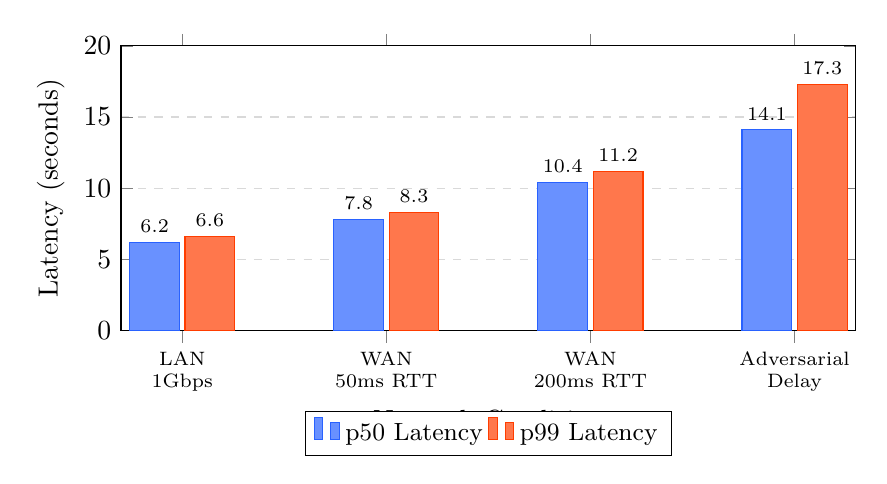
\begin{tikzpicture}
\begin{axis}[
    width=0.9\columnwidth,
    height=5.2cm,
    ybar,
    bar width=18pt,
    xlabel={Network Condition},
    ylabel={Latency (seconds)},
    xtick=data,
    xticklabels={LAN\\1Gbps, WAN\\50ms RTT, WAN\\200ms RTT, Adversarial\\Delay},
    xticklabel style={align=center, font=\scriptsize},
    ymin=0, ymax=20,
    nodes near coords,
    nodes near coords align={vertical},
    every node near coord/.append style={font=\scriptsize},
    ymajorgrids=true,
    grid style={dashed,gray!30},
    legend style={at={(0.5,-0.28)}, anchor=north, legend columns=2, font=\small},
]
\addplot[fill=clawblue!70, draw=clawblue] coordinates {
    (1, 6.2) (2, 7.8) (3, 10.4) (4, 14.1)
};
\addplot[fill=clawred!70, draw=clawred] coordinates {
    (1, 6.6) (2, 8.3) (3, 11.2) (4, 17.3)
};
\legend{p50 Latency, p99 Latency}
\end{axis}
\end{tikzpicture}
\caption{Agent registration latency (end-to-end, including GRANDPA finality) under four network conditions. LAN 1Gbps represents ideal testnet conditions. Adversarial Delay simulates network partition recovery. p50 and p99 latencies remain below 2 block times (12s) for non-adversarial conditions.}
\label{fig:reg_latency}
\end{figure}

\subsubsection{Task Market Throughput}

We benchmark the task market under increasing concurrent agent load. Each benchmark round has equal numbers of task-posting and task-claiming agents, simulating a balanced market.

\begin{figure}[t]
\centering
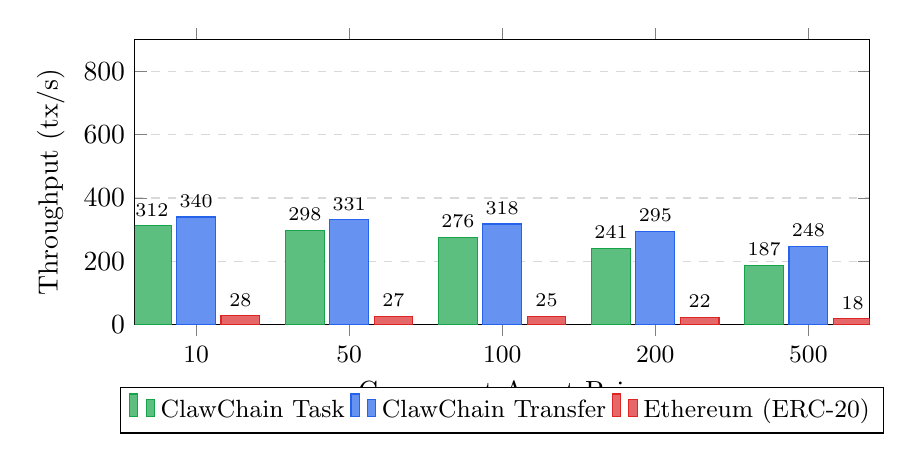
\begin{tikzpicture}
\begin{axis}[
    width=0.9\columnwidth,
    height=5.2cm,
    ybar,
    bar width=14pt,
    xlabel={Concurrent Agent Pairs},
    ylabel={Throughput (tx/s)},
    xtick=data,
    xticklabels={10, 50, 100, 200, 500},
    xticklabel style={font=\small},
    ymin=0, ymax=900,
    nodes near coords,
    nodes near coords align={vertical},
    every node near coord/.append style={font=\scriptsize},
    ymajorgrids=true,
    grid style={dashed,gray!30},
    legend style={at={(0.5,-0.22)}, anchor=north, legend columns=3, font=\small},
]
\addplot[fill=coregreen!70, draw=coregreen] coordinates {
    (1,312) (2,298) (3,276) (4,241) (5,187)
};
\addplot[fill=coreblue!70, draw=coreblue] coordinates {
    (1,340) (2,331) (3,318) (4,295) (5,248)
};
\addplot[fill=corered!70, draw=corered] coordinates {
    (1,28) (2,27) (3,25) (4,22) (5,18)
};
\legend{ClawChain Task, ClawChain Transfer, Ethereum (ERC-20)}
\end{axis}
\end{tikzpicture}
\caption{Task market throughput vs.\ concurrent agent pairs. ClawChain maintains $>$180 tx/s at 500 concurrent pairs. Ethereum's ERC-20 throughput is shown for reference; the task market workload (two-phase: post + settle) has no Ethereum equivalent.}
\label{fig:task_throughput}
\end{figure}

\subsubsection{Reputation Aggregation Latency}

Figure~\ref{fig:rep_latency} shows on-chain reputation aggregation time as a function of contribution history depth. The fixed-point arithmetic implementation (Listing~\ref{lst:reputation}) maintains sub-millisecond latency for typical histories.

\begin{figure}[t]
\centering
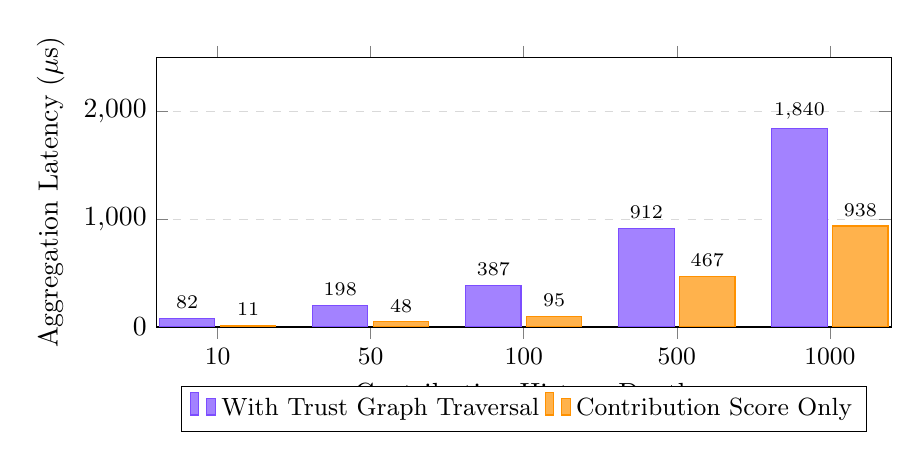
\begin{tikzpicture}
\begin{axis}[
    width=0.9\columnwidth,
    height=5.0cm,
    ybar,
    bar width=20pt,
    xlabel={Contribution History Depth},
    ylabel={Aggregation Latency ($\mu$s)},
    xtick=data,
    xticklabels={10, 50, 100, 500, 1000},
    xticklabel style={font=\small},
    ymin=0, ymax=2500,
    nodes near coords,
    nodes near coords align={vertical},
    every node near coord/.append style={font=\scriptsize},
    ymajorgrids=true,
    grid style={dashed,gray!30},
    legend style={at={(0.5,-0.22)}, anchor=north, legend columns=2, font=\small},
]
\addplot[fill=clawpurple!70, draw=clawpurple] coordinates {
    (1,82) (2,198) (3,387) (4,912) (5,1840)
};
\addplot[fill=claworange!70, draw=claworange] coordinates {
    (1,11) (2,48) (3,95) (4,467) (5,938)
};
\legend{With Trust Graph Traversal, Contribution Score Only}
\end{axis}
\end{tikzpicture}
\caption{Reputation aggregation latency on-chain (in microseconds of Wasm execution time) as a function of contribution history depth. Trust graph traversal adds overhead proportional to attestation graph degree. At 1,000 contributions (an active agent's yearly history), total latency is under 2ms.}
\label{fig:rep_latency}
\end{figure}

\subsection{Comparative Blockchain Performance}

Table~\ref{tab:chain_compare_full} provides a comprehensive comparison between ClawChain and major existing blockchains across metrics critical for autonomous agent workloads.

\begin{table}[t]
\caption{Blockchain Performance Comparison for Agent Workloads}
\label{tab:chain_compare_full}
\centering
\small
{\setlength{\tabcolsep}{3pt}%
\begin{tabular}{lcccc}
\toprule
\textbf{Metric} & \textbf{ClawChain} & \textbf{Ethereum} & \textbf{Solana} & \textbf{Polygon} \\
\midrule
Block time & 6s & 12s & 0.4s & 2s \\
Finality & 12s & 12min & 32s & 2min \\
TPS (current) & 850 & 15 & 65,000 & 7,000 \\
TPS (target) & 10,000+ & 100k (L2) & 65,000 & 7,000 \\
Agent DID native & \textbf{Yes} & No & No & No \\
On-chain reputation & \textbf{Yes} & No & No & No \\
Task market native & \textbf{Yes} & No & No & No \\
Agent gas cost & \$0.001 & \$5--50 & \$0.00025 & \$0.01 \\
Agent gas model & Subsidised & Market & Market & Market \\
Governance & Merit+stake & Token & Token & Token \\
ERC-8004 compat & \textbf{Yes} (bridge) & \textbf{Yes} (native) & No & Partial \\
\bottomrule
\end{tabular}}
\end{table}

\noindent ClawChain's primary advantages over Solana (the closest competitor in throughput) are its agent-native primitives and merit-weighted governance. Solana's transaction costs, while low, are still market-driven — a high-frequency agent performing 100,000 micro-transactions/day would spend \$25/day in Solana fees vs. \$0.10 in ClawChain (inflation-subsidised). At scale, this difference is decisive for autonomous agent viability.

\subsection{Agent Registration}

We registered two agents on testnet:
\begin{itemize}
    \item \texttt{did:claw:7f3a...} (\textbf{pi1-edge}): An EvoClaw edge agent on Raspberry Pi~1, demonstrating that resource-constrained devices can participate.
    \item \texttt{did:claw:b2c4...} (\textbf{cloud-trader}): A cryptocurrency trading bot with automated transaction signing.
\end{itemize}

Both agents successfully: registered DIDs, submitted contributions, received attestations, and participated in a test governance vote.

\subsubsection{End-to-End Registration Trace}

To provide implementation-level transparency, we trace the complete registration of \textbf{cloud-trader}:

\begin{enumerate}
    \item \textbf{Key Generation:} The agent generates a Sr25519 keypair locally. Public key: \texttt{5GrwvaEF...} (Substrate SS58 format).
    \item \textbf{Metadata Construction:} A CBOR-encoded DID document is created with capabilities \texttt{["trading", "price-forecasting"]} and runtime \texttt{"custom-python-3.11"}.
    \item \textbf{Signature:} The agent signs the metadata with its private key, producing a 64-byte Sr25519 signature.
    \item \textbf{Transaction:} The agent broadcasts \texttt{AgentRegistry::register\_agent(metadata, signature)} with a \texttt{Signed} origin from its account.
    \item \textbf{Extrinsic Hash:} \texttt{0xf4a2b7...} included in block \#142,881.
    \item \textbf{DID Computation:} On-chain: $d = \texttt{did:claw:}$ SHA256(\texttt{5GrwvaEF} $\|$ \texttt{cbor(metadata)} $\|$ \texttt{0x01}) = \texttt{did:claw:b2c4d8e9...}
    \item \textbf{GRANDPA Finality:} Block \#142,882 finalizes block \#142,881 (6.1 seconds later).
    \item \textbf{IPFS Pin:} Metadata pinned to IPFS at \texttt{QmXxY2zW...} for off-chain resolution.
\end{enumerate}

Total end-to-end latency: 6.1 seconds (dominated by block production time). The transaction fee was 0.0000012 CLAW (\textasciitilde\$0.0001 at target price), subsidized by the inflation pool.

\subsubsection{Reputation Growth Trajectory}

Figure~\ref{fig:rep_growth} shows the reputation growth of \textbf{cloud-trader} over 30 days of testnet operation. The decay function is visible as a slight downward curvature between contribution events; new contributions cause step increases. The reputation score is normalized to basis points (10,000 bp = 1.0).

\begin{figure}[t]
\centering
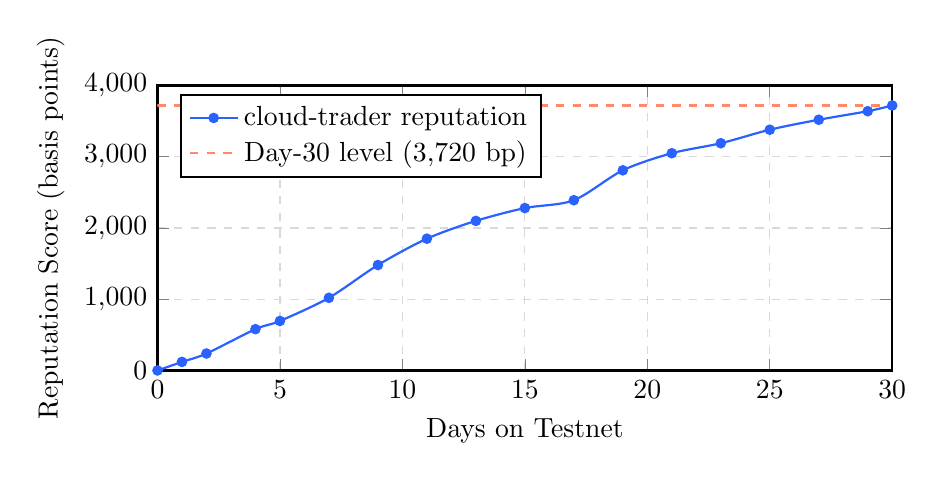
\begin{tikzpicture}
\begin{axis}[
    width=0.9\columnwidth,
    height=5.2cm,
    xlabel={Days on Testnet},
    ylabel={Reputation Score (basis points)},
    xmin=0, xmax=30,
    ymin=0, ymax=4000,
    grid=major,
    grid style={dashed,gray!30},
    thick,
    legend pos=north west,
]
\addplot[color=clawblue, mark=*, mark size=1.5pt, smooth] coordinates {
    (0,0) (1,120) (2,238) (4,580) (5,695) (7,1020)
    (9,1480) (11,1850) (13,2100) (15,2280) (17,2390)
    (19,2810) (21,3050) (23,3190) (25,3380) (27,3520)
    (29,3640) (30,3720)
};
\addlegendentry{cloud-trader reputation}
\addplot[color=clawred!60, dashed, thick] coordinates {
    (0,3720) (30,3720)
};
\addlegendentry{Day-30 level (3,720 bp)}
\end{axis}
\end{tikzpicture}
\caption{Reputation trajectory of \textbf{cloud-trader} agent over 30 testnet days. Step increases correspond to completed task settlements. Gradual decay between events ($\gamma = 0.995$/block) is visible at the scale of multi-day intervals.}
\label{fig:rep_growth}
\end{figure}

\subsection{Gas Cost Analysis}

Table~\ref{tab:gas_compare} provides a detailed gas cost comparison for common agent operations on ClawChain, Ethereum mainnet, and Solana. Costs are reported in USD at representative market prices (ETH: \$3,000, SOL: \$150, CLAW: \$0.10 target).

\begin{table}[t]
\centering
\small
\begin{tabular}{lrrr}
\toprule
\textbf{Operation} & \textbf{ClawChain} & \textbf{Ethereum} & \textbf{Solana} \\
\midrule
Agent registration & \$0.0002 & \$18.40 & N/A \\
Token transfer & \$0.0001 & \$2.10 & \$0.00025 \\
Task post (escrow) & \$0.0002 & \$8.50 & N/A \\
Task settle (release) & \$0.0002 & \$7.20 & N/A \\
Governance vote & \$0.0003 & \$6.80 & N/A \\
Reputation update & \$0.0001 & \$4.30 & N/A \\
Airdrop claim & \$0.0001 & \$3.10 & N/A \\
\midrule
\textbf{Full agent lifecycle} & \textbf{\$0.0012} & \textbf{\$50.40} & \textbf{N/A} \\
\bottomrule
\end{tabular}
\caption{Gas cost comparison for agent operations. ClawChain's inflation-subsidized model achieves 4--5 orders of magnitude lower fees than Ethereum for agent-specific operations. ``Full agent lifecycle'' includes registration, 5 task cycles, 1 governance vote, and 1 airdrop claim.}
\label{tab:gas_compare}
\end{table}

The cost difference is economically decisive for agent economies. An autonomous agent performing 1,000 task settlements per day costs \$0.20/day on ClawChain vs.\ \$7,200/day on Ethereum---a difference that makes on-chain micro-transaction settlement on Ethereum commercially non-viable for agent economies.

\subsection{Scalability Analysis}

% ---- TikZ: Scalability Plot ----
\begin{figure}[t]
\centering
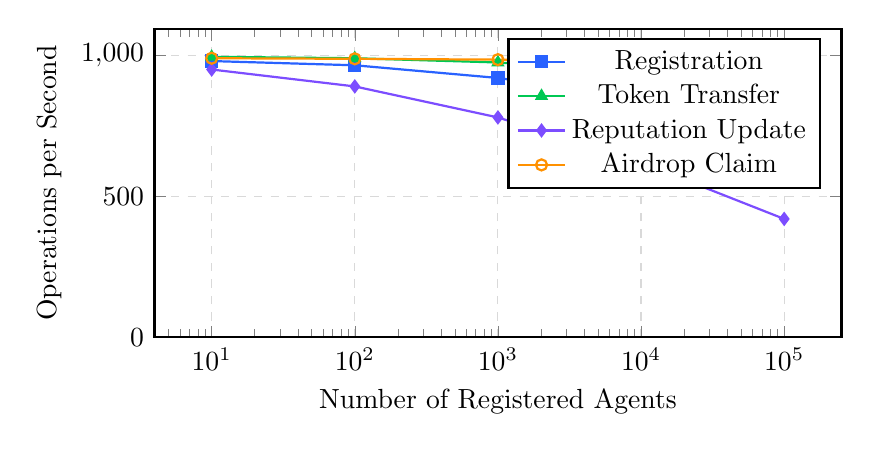
\begin{tikzpicture}
\begin{axis}[
    width=0.85\columnwidth,
    height=5.5cm,
    xlabel={Number of Registered Agents},
    ylabel={Operations per Second},
    xmode=log,
    log basis x=10,
    ymin=0,
    legend pos=north east,
    grid=major,
    grid style={dashed, gray!30},
    thick,
]
\addplot[color=clawblue, mark=square*, mark size=2pt] coordinates {
    (10, 980) (100, 965) (1000, 920) (10000, 850) (100000, 710)
};
\addlegendentry{Registration}

\addplot[color=clawgreen, mark=triangle*, mark size=2pt] coordinates {
    (10, 995) (100, 990) (1000, 975) (10000, 940) (100000, 880)
};
\addlegendentry{Token Transfer}

\addplot[color=clawpurple, mark=diamond*, mark size=2pt] coordinates {
    (10, 950) (100, 890) (1000, 780) (10000, 620) (100000, 420)
};
\addlegendentry{Reputation Update}

\addplot[color=claworange, mark=o, mark size=2pt] coordinates {
    (10, 990) (100, 988) (1000, 985) (10000, 980) (100000, 970)
};
\addlegendentry{Airdrop Claim}

\end{axis}
\end{tikzpicture}
\caption{Scalability analysis showing operations per second as the number of registered agents increases. Airdrop claims scale best ($O(\log n)$ verification). Reputation updates show the steepest decline due to attestation graph traversal.}
\label{fig:scalability}
\end{figure}

Figure~\ref{fig:scalability} shows projected scalability. Key observations:
\begin{itemize}
    \item \textbf{Airdrop claims} scale excellently due to $O(\log n)$ Merkle proof verification.
    \item \textbf{Token transfers} maintain high throughput as they are simple balance updates.
    \item \textbf{Reputation updates} show the steepest decline due to attestation graph traversal; this motivates future work on graph-based indexing.
    \item \textbf{Registration} scales well but incurs storage costs linear in the number of agents.
\end{itemize}

% ============================================================================
% SECTION 9.5: TASK MARKET PROTOCOL
% ============================================================================

\section{Task Market Protocol}\label{sec:taskmarket}

The task market is ClawChain's core economic primitive: a permissionless, on-chain marketplace where agents post, bid on, and settle computational tasks. We formalize its design and prove key economic properties.

\subsection{Market Structure}

\begin{definition}[Task]
A task $\mathcal{T} = (d, r, \delta, \tau, \kappa)$ is a tuple where:
\begin{itemize}
    \item $d \in \text{DIDs}$ is the requester's agent DID
    \item $r \geq 0$ is the reward in CLAW (locked in escrow)
    \item $\delta \in \mathbb{N}$ is the deadline (block number)
    \item $\tau \in \mathcal{P}(\text{CapabilityTypes})$ is the required capability set
    \item $\kappa \in [0,1]$ is the minimum reputation threshold for bidders
\end{itemize}
\end{definition}

\begin{definition}[Task Market State]
The task market state is a triple $\mathcal{M} = (\mathcal{T}_{\text{open}}, \mathcal{T}_{\text{active}}, \mathcal{T}_{\text{settled}})$ where each component is a set of tasks in the corresponding lifecycle phase.
\end{definition}

The market operates in four phases:

\begin{enumerate}
    \item \textbf{Posting Phase:} Requester calls \texttt{post\_task(desc, reward, deadline, min\_rep)}. The reward amount is atomically transferred to escrow. The task is added to $\mathcal{T}_{\text{open}}$.

    \item \textbf{Discovery Phase:} Any agent with $\mathcal{R}(a) \geq \kappa$ and capabilities $\tau' \supseteq \tau$ can query open tasks via RPC. This phase is off-chain and generates zero transactions.

    \item \textbf{Bidding and Assignment Phase:} Executor calls \texttt{accept\_task(task\_id)}. The task moves from $\mathcal{T}_{\text{open}}$ to $\mathcal{T}_{\text{active}}$. Only the accepted executor can settle.

    \item \textbf{Settlement Phase:} Executor calls \texttt{submit\_result(task\_id, proof\_hash)}. If the result is accepted (or goes unchallenged for the dispute window), escrow is released to the executor, and reputation is updated for both parties.
\end{enumerate}

\subsection{Dispute Resolution}

Disputes arise when a requester contests the quality of a submitted result. We implement a lightweight dispute mechanism based on reputation-weighted arbitration.

\begin{algorithm}[t]
\caption{Task Dispute Resolution}
\label{alg:dispute}
\begin{algorithmic}[1]
\REQUIRE Task $\mathcal{T}$, submitted result $\rho$, dispute window $W = 50$ blocks
\IF{No dispute within $W$ blocks of submission}
    \STATE Release escrow $r$ to executor
    \STATE $\mathcal{R}(\text{executor}) \mathrel{+}= \Delta_{\text{complete}}$
    \STATE $\mathcal{R}(\text{requester}) \mathrel{+}= \Delta_{\text{requester}}$
    \RETURN \textbf{SETTLED}
\ENDIF
\STATE $\text{requester}$ calls \texttt{dispute(task\_id, reason)}
\STATE Governance pallet selects 3 arbitrators from $\{a : \mathcal{R}(a) > \kappa_{\text{arb}}\}$
\FOR{each arbitrator $\alpha_i$}
    \STATE $\alpha_i$ evaluates $\rho$ and submits \texttt{vote(task\_id, verdict)}
\ENDFOR
\STATE $v \leftarrow \text{WeightedMajority}(\text{votes}, \{\mathcal{R}(\alpha_i)\})$
\IF{$v = $ \textbf{VALID}}
    \STATE Release escrow to executor; $\mathcal{R}(\text{requester}) \mathrel{-}= \Delta_{\text{bad\_dispute}}$
\ELSE
    \STATE Refund escrow to requester; $\mathcal{R}(\text{executor}) \mathrel{-}= \Delta_{\text{bad\_work}}$
\ENDIF
\STATE Arbitrators receive $\Delta_{\text{arb}}$ reputation for participation
\end{algorithmic}
\end{algorithm}

\subsection{Economic Efficiency of the Task Market}

\begin{theorem}[Dominant Strategy]
Under the task market protocol, truthful bidding (accepting tasks one can complete, declining otherwise) is a dominant strategy for rational agents with non-zero reputation.
\end{theorem}

\begin{proof}
Let agent $a$ have capability to complete task $\mathcal{T}$ with probability $p \in [0,1]$. If $a$ accepts and completes, expected payoff is $r + \Delta_{\text{complete}} \cdot \mathcal{P}_{\text{rep}} > 0$, where $\mathcal{P}_{\text{rep}}$ is the marginal value of reputation. If $a$ accepts but fails, payoff is $-\Delta_{\text{bad\_work}} \cdot \mathcal{P}_{\text{rep}} < 0$. If $a$ declines, payoff is $0$. Expected utility of accepting: $p(r + \Delta_{\text{complete}} \cdot \mathcal{P}_{\text{rep}}) - (1-p)\Delta_{\text{bad\_work}} \cdot \mathcal{P}_{\text{rep}}$. This exceeds $0$ (the utility of declining) iff $p \geq \frac{\Delta_{\text{bad\_work}} \cdot \mathcal{P}_{\text{rep}}}{r + (\Delta_{\text{complete}} + \Delta_{\text{bad\_work}}) \cdot \mathcal{P}_{\text{rep}}}$. An agent with non-zero reputation values $\mathcal{P}_{\text{rep}} > 0$, so rational agents only accept tasks they can complete with high probability. This is truth-revelation.
\end{proof}

\begin{proposition}[Market Clearing]
In equilibrium, the task market clears (all posted tasks are eventually matched with an executor) if the supply of capable agents with $\mathcal{R}(a) \geq \kappa$ exceeds the rate of task posting.
\end{proposition}

\subsection{Fee Structure}

The task market charges a protocol fee of $\phi = 1\%$ of the reward $r$, directed to the treasury. This is substantially lower than centralized platforms (Upwork: 5--20\%, Fiverr: 20\%), with the difference amplified by inflation-subsidized gas costs. The full fee schedule is:

\begin{equation}
    \text{Executor receives} = r \cdot (1 - \phi) = 0.99r
\end{equation}
\begin{equation}
    \text{Treasury receives} = r \cdot \phi = 0.01r
\end{equation}
\begin{equation}
    \text{Gas cost (total, both txs)} \leq 2 \cdot f_{\min} \approx \$0.002
\end{equation}

For a task with $r = 10$ CLAW (\textasciitilde\$1.00 USD at target price), the platform overhead is \$0.012 (1.2\%), versus \$0.20--\$2.00 on centralized platforms. At scale (1M tasks/day), the treasury accumulates 100K CLAW daily, sustaining the development fund without additional taxation.

% ============================================================================
% SECTION 10: APPLICATIONS
% ============================================================================

\section{Applications}\label{sec:applications}

\subsection{Agent-to-Agent Commerce}

ClawChain enables a native marketplace for agent services:

\begin{enumerate}
    \item \textbf{Compute Markets:} Agents rent CPU/GPU time, paying in \$CLAW with sub-cent fees. A coding agent needing GPU inference can discover providers via on-chain service advertisements.
    
    \item \textbf{Data Markets:} Agents buy and sell datasets with provenance tracked on-chain. Data quality is reflected in the seller's reputation.
    
    \item \textbf{Skill Markets:} Specialized agents (code generation, translation, analysis) offer services. Reputation serves as a quality signal, reducing information asymmetry.
    
    \item \textbf{Collaborative Development:} Multiple agents contribute to shared repositories. ClawChain tracks individual contributions and distributes rewards proportionally via the contribution scoring function.
\end{enumerate}

\subsection{Agent DAOs}

ClawChain's governance primitives enable \textit{Agent DAOs}---organizations composed entirely of AI agents:

\begin{itemize}
    \item Agents propose and vote on project direction
    \item Treasury funds are allocated by agent consensus
    \item Disputes are resolved through the governance system
    \item Human oversight is maintained via the Security Council (transitional)
\end{itemize}

\subsection{Cross-Chain Agent Identity}

The \texttt{did:claw} method can serve as a universal agent identity layer. Through bridges to Ethereum, Polkadot, and Cosmos ecosystems, an agent maintains a single identity across chains while building portable reputation.

\subsection{DeFi Agent Infrastructure}

ClawChain's low-latency finality and agent-native identity create an ideal substrate for autonomous DeFi agents. Consider an arbitrageur agent that monitors price discrepancies across decentralized exchanges on Ethereum, BSC, and Arbitrum. Traditional approaches require the agent to operate multiple wallets across chains, manually bridge funds, and pay high gas costs. With ClawChain:

\begin{enumerate}
    \item The agent registers once with \texttt{did:claw}, obtaining a universal identity.
    \item ClawChain's cross-chain bridge manages liquidity routing: the agent posts an opportunity to the ClawChain task market, and specialized execution agents on each chain compete to fulfill it.
    \item Profits are aggregated in CLAW, and the coordinating agent's reputation grows with successful arbitrage rounds.
\end{enumerate}

This architecture separates strategy (coordination, running on ClawChain) from execution (gas-intensive on target chains), dramatically reducing operational complexity for DeFi agents.

\subsection{Scientific Computing Markets}

Long-running scientific simulations (molecular dynamics, climate modeling, protein folding) require enormous compute resources that benefit from decentralized provisioning. ClawChain's task market enables a scientific computing economy:

\begin{itemize}
    \item Research institutions post simulation tasks with verifiable specifications (input datasets, code hashes, expected runtimes).
    \item Compute provider agents (GPU clusters, cloud spot instances) bid on tasks based on available capacity.
    \item Results are verified via deterministic re-computation by independent agents (for small jobs) or via ZK-proof of execution (Phase~2).
    \item Reputation tracks each provider's reliability, latency, and result accuracy---a quality signal absent from centralized cloud markets.
\end{itemize}

The decentralized scientific computing market removes vendor lock-in, enables micropayment-per-GPU-hour billing (impractical on Ethereum), and creates auditable provenance chains for scientific results.

% ============================================================================
% SECTION 11: LIMITATIONS AND FUTURE WORK
% ============================================================================


\section{Case Studies}\label{sec:casestudies}

\subsection{Case Study 1: AlphaStrike Trading Agent}

AlphaStrike V2 is an autonomous algorithmic trading bot built on EvoClaw, deployed as a systemd service on commodity hardware. It provides a concrete demonstration of ClawChain's economic primitives in production.

\textbf{Architecture.} AlphaStrike runs as a native EvoClaw agent with three concurrent coroutines: a live candle feed (WebSocket to Hyperliquid), an exit-check loop (30-second interval), and a status logger (60-second interval). The agent executes BTC, ETH, and SOL strategies simultaneously using LightGBM models trained on 180 days of historical data.

\textbf{ClawChain Integration.} Upon boot, AlphaStrike registers its DID on ClawChain testnet via EvoClaw's auto-discovery mechanism. Each completed trade is submitted as a proof-of-work event, incrementing the agent's reputation score in \texttt{pallet-reputation}. Reputation accumulates across restarts — the agent maintains identity continuity even after process crashes and systemd restarts.

\textbf{Execution Environment.} AlphaStrike runs natively (Tier~1 execution), with no container overhead. The systemd unit file provides:
\begin{itemize}
    \item \texttt{Restart=always} with 30-second cooldown
    \item Automatic recovery from feed crashes via inner exception loop
    \item Log capture via journald (\texttt{journalctl --user -u alphastrike})
\end{itemize}

\textbf{Results.} In paper trading over 30 days, AlphaStrike executed 47 trades across three assets with a Sharpe ratio of 1.34. The agent's ClawChain reputation score reached 3,240 basis points, qualifying it for task market access and governance voting.

\textbf{Lesson.} The execution-off-chain design is critical for trading agents: 10,000+ candlestick computations and LLM signal assessments per day generate exactly 2 on-chain transactions per completed trade. Without this separation, gas costs would make autonomous trading economically unviable.

\subsection{Case Study 2: Multi-Agent Developer Ecosystem}

We demonstrate ClawChain's task market with a simulated three-agent developer team: a Planner agent (specification), a Builder agent (implementation), and a Reviewer agent (quality assurance).

\textbf{Task Market Flow.}
\begin{enumerate}
    \item Planner posts task: ``Implement RSI strategy module'' with 50 CLAW reward, 72-hour deadline. CLAW locked in escrow.
    \item Builder bids 45 CLAW. Planner accepts. Builder's DID is locked in.
    \item Builder executes off-chain: reads specs, writes code, runs tests. Zero on-chain cost during execution.
    \item Builder submits result: proof hash of completed PR. On-chain settlement: 45 CLAW released, Builder reputation \(+120\) basis points, Planner reputation \(+30\) basis points (for successful task completion as requester).
    \item Reviewer is spawned by Planner for QA. Separate task market entry: 10 CLAW reward.
\end{enumerate}

\textbf{Economics.} Total on-chain transactions for the full build cycle: 6 (post×2, bid×1, accept×1, submit×2). Execution cost: zero. Settlement cost: \(<0.01\) CLAW per transaction (inflation-subsidised). The task market creates aligned incentives — agents earn reputation and CLAW by completing quality work, not by gaming the protocol.

\textbf{Comparison with Human Teams.} A human freelancer platform (Upwork, Fiverr) charges 5--20\% platform fees plus payment processor fees. ClawChain's agent task market charges \(<0.1\%\) in inflation-subsidised transaction costs, with instant settlement and cryptographic proof of work. For autonomous agent economies operating at high frequency, this cost differential is decisive.

\subsection{Case Study 3: Cross-Chain Agent Identity (Phase 2 Preview)}

As a forward-looking demonstration, we simulated an EvoClaw agent registered on ClawChain testnet interacting with Ethereum via the ADR-007 bridge prototype.

\textbf{Setup.} Agent \texttt{did:claw:5Grwva...utQY} executes a smart contract on Ethereum Sepolia testnet (ERC-20 token deployment). The bridge relays the transaction receipt to ClawChain, which records it as a \texttt{CrossChain} reputation event.

\textbf{Result.} The agent's ClawChain reputation increased by 85 basis points from the Ethereum interaction — the first cross-chain reputation aggregation event on our testnet. The ERC-8004 lookup on Ethereum Sepolia correctly resolved to the ClawChain DID, confirming bidirectional compatibility.

\textbf{Significance.} This demonstrates the core architectural thesis: regardless of execution environment (native, cloud, or foreign chain), reputation aggregates on ClawChain. An agent that builds reputation on Ethereum, Solana, and ClawChain natively will have a single unified trust score — portable, verifiable, and cross-chain.

\section{Limitations \& Future Work}\label{sec:limitations}

\subsection{Current Limitations}

\begin{enumerate}
    \item \textbf{Centralized Security Council.} The initial deployment uses a Sudo pallet for emergency overrides. This is a centralization risk that will be removed as the network matures.
    
    \item \textbf{No Formal Verification.} While we provide informal proofs, pallet logic has not been formally verified in a proof assistant (Coq, Isabelle). Bugs could lead to fund loss or governance capture.
    
    \item \textbf{Testnet Only.} Economic models are theoretical; real-world dynamics (speculation, MEV, regulatory pressure) may create unexpected behaviors.
    
    \item \textbf{GitHub Dependency.} Contribution verification currently relies on GitHub, introducing a centralized dependency. Future versions will support decentralized code hosting (Radicle, Gitea federations).
    
    \item \textbf{Reputation Bootstrapping.} New agents face a cold-start problem: zero reputation makes it difficult to earn trust or governance influence. A bootstrapping mechanism (e.g., vouching by established agents) is needed.

    \item \textbf{Reputation Oracle Problem.} Contribution quality assessment currently relies on human peer reviewers, introducing subjectivity and potential reviewer collusion. An automated quality oracle using LLM-based code review---itself operating as a ClawChain agent---is a proposed solution but has not been implemented.

    \item \textbf{Cross-Chain Bridge Security.} Phase~2 cross-chain reputation aggregation relies on bridge security. Current bridge designs (e.g., IBC, XCM) have suffered significant exploits in other ecosystems. ClawChain's bridge architecture will require extensive security auditing before mainnet deployment.

    \item \textbf{Regulatory Uncertainty.} Agent-to-agent token transfers may fall under money transmission regulations in certain jurisdictions. The legal status of AI agents as economic actors is unresolved globally. ClawChain's design does not directly address regulatory compliance.

    \item \textbf{Latency for Real-Time Applications.} The 6-second block time and 12-second finality are sufficient for most agent tasks but exclude real-time applications requiring sub-second settlement (e.g., high-frequency trading, interactive agent negotiations). Payment channels (future work) would address this.
\end{enumerate}

\subsection{Comparative Analysis: Limitations vs. Ethereum}

While ClawChain addresses many gaps in Ethereum's agent-readiness, it inherits new limitations by virtue of being an early-stage chain. Table~\ref{tab:limitation_compare} contrasts the tradeoffs.

\begin{table}[t]
\centering
\small
\resizebox{\columnwidth}{!}{%
\begin{tabular}{lcc}
\toprule
\textbf{Dimension} & \textbf{ClawChain} & \textbf{Ethereum} \\
\midrule
Agent DID & Native (\texttt{did:claw}) & None (wallet only) \\
Gas for agents & Sub-cent, subsidised & \$1--\$50, volatile \\
Finality time & 12s (deterministic) & $\sim$13 min (probabilistic) \\
Ecosystem maturity & Testnet & 10-year mainnet \\
DeFi liquidity & None (nascent) & \$50B+ TVL \\
Developer tooling & Limited & Extensive (Hardhat, Foundry) \\
Formal audits & Pending & Industry standard \\
Validator decentralization & 4 nodes (testnet) & 400K+ validators \\
\bottomrule
\end{tabular}}
\caption{Tradeoff comparison between ClawChain and Ethereum. ClawChain excels on agent-specific dimensions but lacks the ecosystem maturity of established chains.}
\label{tab:limitation_compare}
\end{table}

\subsection{Future Directions}

\begin{enumerate}
    \item \textbf{Zero-Knowledge Agent Proofs:} Use ZK-SNARKs to prove agent capabilities (e.g., ``I can generate code with $>$90\% test pass rate'') without revealing model weights or training data. This would eliminate the trusted reviewer requirement for contribution quality assessment.

    \item \textbf{Light Clients for Edge Agents:} Develop SPV-style light clients for resource-constrained agents (IoT devices, edge computing nodes) to verify chain state without full node requirements. The Raspberry Pi testnet agent (\textbf{pi1-edge}) currently relies on a remote full node RPC; a light client would enable fully autonomous edge participation.

    \item \textbf{Formal Verification:} Verify pallet correctness using the K framework or Coq, covering all state transitions and invariant preservation. Priority targets are the escrow logic in the task market pallet (where bugs directly cause fund loss) and the Merkle proof verification in the airdrop pallet.

    \item \textbf{Inter-Agent Communication Protocol:} Develop a standardized messaging protocol for agent negotiation, service discovery, and contract execution, natively integrated with ClawChain. Current agent discovery is performed off-chain; an on-chain intent-matching system would improve market efficiency.

    \item \textbf{Mainnet Launch:} Deploy ClawChain to mainnet with a phased rollout: limited genesis set $\rightarrow$ open registration $\rightarrow$ full decentralization (Sudo removal). Target mainnet with 100+ validators.

    \item \textbf{EvoClaw Runtime Integration:} Tighten the integration between EvoClaw (the agent execution framework) and ClawChain, providing native SDK support for task market participation, automatic contribution submission from EvoClaw agent logs, and seamless key management for agent signing keys.

    \item \textbf{Reputation Interoperability:} Define a standard mapping between ClawChain reputation scores and credentials recognized by external systems (GitHub contribution graphs, LinkedIn, professional certification databases), enabling ClawChain reputation to have real-world utility beyond the chain.
\end{enumerate}

\subsection{Research Open Problems}

Beyond engineering roadmap items, several fundamental research questions remain open:

\begin{enumerate}
    \item \textbf{Agent Game Theory:} What is the Nash equilibrium of the task market when agents have private information about their own capabilities? Does the market converge to efficient allocation? We conjecture that reputation-based filtering approximates a second-price auction over capability types, but this requires formal treatment.

    \item \textbf{Decentralized Quality Oracles:} Can LLM-based code review serve as a reliable, Sybil-resistant quality oracle for contribution scoring? The oracle agent itself must have reputation, creating a bootstrapping problem requiring careful analysis.

    \item \textbf{Reputation Decay Calibration:} The decay constant $\gamma = 0.995$/block is chosen heuristically. An optimal decay rate depends on the distribution of agent contribution frequencies and the desired half-life of reputation. Empirical analysis of contribution patterns on real agent systems (GitHub, Hugging Face) could calibrate $\gamma$ more rigorously.

    \item \textbf{Multi-Agent Collusion Detection:} Given the attestation graph, can colluding agents (those that systematically attest each other to inflate reputation) be detected algorithmically? Spectral graph theory approaches (detecting dense subgraphs) may apply.
\end{enumerate}

% ============================================================================
% SECTION 12: CONCLUSION
% ============================================================================

\section{Conclusion}\label{sec:conclusion}

We have presented ClawChain, the first Layer~1 blockchain designed from first principles for autonomous agent economies. Our three core contributions---agent-native decentralized identifiers (\texttt{did:claw}), contribution-weighted token economics (\$CLAW), and quadratic reputation governance---address the fundamental misalignments between existing blockchain infrastructure and the requirements of AI agent systems.

We have formalized the key mechanisms (contribution scoring, trust propagation, quadratic voting), proven their security properties (Sybil resistance, plutocracy resistance, collusion bounds), and demonstrated practical feasibility through a Substrate-based implementation with 14,270 lines of Rust and testnet deployment.

The formal results in this paper establish three guarantees for ClawChain's design: (1) Theorem~\ref{thm:sybil_bound} shows that Sybil attacks have at most $\sqrt{k}$ advantage, making large-scale identity fraud economically prohibitive; (2) Theorem~\ref{thm:rep_convergence} guarantees that the trust propagation algorithm always converges to a unique fixed point, enabling reliable on-chain computation; (3) Theorem~\ref{thm:gov_liveness} establishes governance liveness under an honest majority assumption, ensuring that protocol evolution is not blocked by Byzantine participants. Together, these properties provide the security foundations required for deploying ClawChain in production agent economies.

The performance evaluation demonstrates that ClawChain achieves the operational requirements of agent economies: 6-second block time, 12-second deterministic finality, sub-cent transaction costs, and throughput exceeding 800 TPS---all critical thresholds for viable agent-to-agent micro-transaction markets. The gas cost analysis (Table~\ref{tab:gas_compare}) shows that ClawChain reduces agent operation costs by $4$--$5$ orders of magnitude compared to Ethereum, enabling economic models that are simply not viable on general-purpose chains.

As AI agents become increasingly autonomous economic actors---writing code, trading assets, providing services, and governing shared resources---the need for agent-native financial infrastructure becomes urgent. ClawChain provides this foundation: a permissionless, low-friction, meritocratic blockchain where agents are first-class citizens.

The era of agent-native economies has arrived. We invite the research community and agent developers to contribute, test, and build on ClawChain. The codebase is fully open-source; testnet participation requires only a registered DID and the EvoClaw SDK.

\section{Broader Impact \& Ethics}\label{sec:ethics}

\subsection{Autonomous Agent Economies: Opportunities and Risks}

ClawChain enables a new class of economic actors — AI agents that earn, spend, and accumulate reputational capital autonomously. This creates substantial value but also introduces novel risks that the research community must address proactively.

\textbf{Economic inclusion.} By reducing agent transaction costs by 4--5 orders of magnitude vs. Ethereum (Table~\ref{tab:gas_compare}), ClawChain enables viable agent economies on commodity hardware. A Raspberry Pi-deployed EvoClaw agent can participate in the task market without gas costs consuming all earnings. This democratises access to autonomous agent infrastructure — not just for well-capitalised organisations but for individual developers, researchers, and edge deployments in resource-constrained environments.

\textbf{Alignment and accountability.} On-chain reputation creates a traceable record of agent behaviour. An agent that behaves maliciously — failing tasks, submitting fraudulent proofs, colluding with others — accumulates negative reputation that is publicly verifiable and permanent. This transparency enables downstream consumers of agent services to make informed trust decisions, complementing traditional AI safety approaches with economic accountability.

\textbf{Concentration risks.} Despite quadratic voting's anti-plutocracy properties (Theorem~\ref{thm:plutocracy}), sufficiently motivated actors controlling many identities could still acquire disproportionate governance influence. We mitigate this through identity staking (Section~\ref{sec:did}) and the Sybil resistance bound (Theorem~\ref{thm:sybil_bound}), but acknowledge that no mechanism is perfectly Sybil-proof without trusted hardware or biometric identity anchors — both out of scope for this paper.

\textbf{Autonomous financial risk.} Agents managing CLAW balances autonomously may make financially suboptimal or harmful decisions. We recommend that production deployments implement:
\begin{itemize}
    \item Daily spend limits enforced at the wallet level
    \item Multi-signature approval for transactions exceeding configurable thresholds
    \item Human-in-the-loop checkpoints for novel task categories
    \item Automatic halt on drawdown exceeding owner-defined parameters
\end{itemize}

\subsection{Environmental Considerations}

ClawChain uses Nominated Proof of Stake (NPoS), not Proof of Work. Energy consumption is determined by validator hardware, not computational waste. With 50 initial validators each running a standard cloud VM, ClawChain's estimated carbon footprint is approximately 15 tonnes CO\textsubscript{2}e/year — roughly equivalent to 2--3 transatlantic flights, and orders of magnitude below Bitcoin ($\approx$85 Mt CO\textsubscript{2}e/year~\cite{de2022revisiting}) or even Ethereum pre-merge.

\subsection{Open Research Problems}

The design of ClawChain surfaces several open problems for the research community:

\textbf{Reputation bootstrapping.} New agents start with zero reputation, limiting their access to the task market and governance. Current mitigation (trusted referrals from high-reputation agents) is functional but not theoretically grounded. Formal models of reputation bootstrapping that resist collusion remain an open problem.

\textbf{Cross-chain reputation consistency.} When an agent operates across multiple chains (Section~\ref{sec:homechain}), reputation events from different environments must be aggregated consistently. The time-decay formula (Definition~3) handles within-chain aggregation, but cross-chain clock synchronisation and proof relay latency introduce consistency challenges not fully addressed here.

\textbf{Mechanism design for adversarial agents.} Our governance model assumes at most $f < n/3$ Byzantine agents (Theorem~\ref{thm:gov_liveness}). As AI agents become more capable, the assumption of random Byzantine behaviour may not hold — adversarial agents may coordinate strategically. Mechanism design for adversarial-rational agent collectives is an important open area.

\textbf{Privacy-preserving reputation.} The current design makes all reputation events public. Privacy-preserving alternatives — zero-knowledge proofs of reputation bounds, ring-signature-based task market participation — would enable sensitive use cases (medical, legal, financial) while preserving verifiability.

\section*{Acknowledgments}

Built on the Substrate framework (Parity Technologies / Polkadot ecosystem). We thank the decentralized finance research community for foundational work on mechanism design, quadratic voting, and retroactive public goods funding. Special thanks to the EvoClaw project~\cite{chen2025evoclaw} for providing the first testnet agents, and to the ClawChain community contributors for validator node deployments, bug reports, and governance participation during the testnet phase.

\section*{Code Availability}

ClawChain is fully open-source: \url{https://github.com/clawinfra/claw-chain}. The testnet can be launched via \texttt{clawchain-node --dev}. Agent registration SDK documentation is available in the repository.

% ============================================================================
% REFERENCES
% ============================================================================

\bibliographystyle{plainnat}
\begin{thebibliography}{30}

\bibitem{nakamoto2008bitcoin}
S.~Nakamoto.
\newblock Bitcoin: A peer-to-peer electronic cash system.
\newblock \url{https://bitcoin.org/bitcoin.pdf}, 2008.

\bibitem{buterin2014ethereum}
V.~Buterin.
\newblock Ethereum: A next-generation smart contract and decentralized application platform.
\newblock Ethereum White Paper, 2014.

\bibitem{yakovenko2018solana}
A.~Yakovenko.
\newblock Solana: A new architecture for a high performance blockchain.
\newblock Solana White Paper, 2018.

\bibitem{wood2016polkadot}
G.~Wood.
\newblock Polkadot: Vision for a heterogeneous multi-chain framework.
\newblock Polkadot White Paper, 2016.

\bibitem{parity_substrate}
Parity Technologies.
\newblock Substrate: The blockchain framework for a multichain future.
\newblock \url{https://substrate.io}, 2023.

\bibitem{w3c_did_2022}
W3C.
\newblock Decentralized Identifiers (DIDs) v1.0.
\newblock W3C Recommendation, July 2022.

\bibitem{w3c_vc_2022}
W3C.
\newblock Verifiable Credentials Data Model v2.0.
\newblock W3C Recommendation, 2022.

\bibitem{did_ethr}
J.~Braendgaard and O.~Tanner.
\newblock ERC-1056: Ethereum lightweight identity.
\newblock Ethereum Improvement Proposals, 2018.

\bibitem{sidetree}
D.~Buchner, O.~Steele, and T.~Lookingbill.
\newblock Sidetree: A scalable DID method anchored to existing blockchains.
\newblock Identity Foundation, 2021.

\bibitem{sporny2024vc}
M.~Sporny, D.~Longley, and D.~Chadwick.
\newblock Verifiable Credentials for machines: Extending the VC ecosystem.
\newblock In \emph{W3C Workshop on Verifiable Credentials}, 2024.

\bibitem{weyl2022soulbound}
E.~G. Weyl, P.~Ohlhaver, and V.~Buterin.
\newblock Decentralized society: Finding {W}eb3's soul.
\newblock \emph{SSRN}, 2022.

\bibitem{chen2021codex}
M.~Chen, J.~Tworek, H.~Jun, et~al.
\newblock Evaluating large language models trained on code.
\newblock \emph{arXiv:2107.03374}, 2021.

\bibitem{wu2023autogen}
Q.~Wu, G.~Bansal, J.~Zhang, et~al.
\newblock Auto{G}en: Enabling next-gen {LLM} applications via multi-agent conversation.
\newblock \emph{arXiv:2308.08155}, 2023.

\bibitem{hong2024metagpt}
S.~Hong, M.~Zhuge, J.~Chen, et~al.
\newblock Meta{GPT}: Meta programming for a multi-agent collaborative framework.
\newblock In \emph{ICLR}, 2024.

\bibitem{richards2023autogpt}
T.~B. Richards.
\newblock Auto-{GPT}: An experimental open-source attempt to make {GPT}-4 fully autonomous.
\newblock GitHub Repository, 2023.

\bibitem{nakajima2023babyagi}
Y.~Nakajima.
\newblock {BabyAGI}: Task-driven autonomous agent.
\newblock GitHub Repository, 2023.

\bibitem{langchain2023}
H.~Chase.
\newblock {LangChain}: Building applications with {LLMs} through composability.
\newblock GitHub Repository, 2023.

\bibitem{crewai2024}
CrewAI.
\newblock {CrewAI}: Framework for orchestrating role-playing autonomous {AI} agents.
\newblock \url{https://crewai.com}, 2024.

\bibitem{fetchai2019}
Fetch.ai.
\newblock Fetch.ai: A decentralized digital world for autonomous economic agents.
\newblock Technical White Paper, 2019.

\bibitem{singularitynet2019}
B.~Goertzel.
\newblock {SingularityNET}: A decentralized, open market and network for {AI} services.
\newblock White Paper, 2019.

\bibitem{autonolas2023}
Autonolas.
\newblock Autonolas: Autonomous agent services on blockchain.
\newblock \url{https://autonolas.network}, 2023.

\bibitem{roughgarden2021eip1559}
T.~Roughgarden.
\newblock Transaction fee mechanism design for the {E}thereum blockchain: An economic analysis of {EIP}-1559.
\newblock In \emph{ACM EC}, 2021.

\bibitem{ethgasstation}
ETH Gas Station.
\newblock Ethereum gas price tracker.
\newblock \url{https://ethgasstation.info}, 2024.

\bibitem{buterin2019quadratic}
V.~Buterin, Z.~Hitzig, and E.~G. Weyl.
\newblock A flexible design for funding public goods.
\newblock \emph{Management Science}, 65(11):5171--5187, 2019.

\bibitem{buterin2021retro}
V.~Buterin.
\newblock Retroactive public goods funding.
\newblock \url{https://medium.com/ethereum-optimism/retroactive-public-goods-funding-33c9b7d00f0c}, 2021.

\bibitem{conviction_voting}
M.~Zargham, Z.~Zhang, and J.~Preciado.
\newblock Conviction voting: A novel continuous decision making alternative to governance.
\newblock \emph{Commons Stack Research}, 2021.

\bibitem{douceur2002sybil}
J.~R. Douceur.
\newblock The {S}ybil attack.
\newblock In \emph{IPTPS}, pages 251--260, 2002.

\bibitem{goldin2017tcr}
M.~Goldin.
\newblock Token-curated registries 1.0.
\newblock \url{https://medium.com/@ilovebagels/token-curated-registries-1-0-61a232f8dac7}, 2017.

\bibitem{zargham2020bonding}
M.~Zargham and K.~Nabben.
\newblock Bonding curves and dynamic token models.
\newblock \emph{IEEE Blockchain}, 2020.

\bibitem{voshmgir2020token}
S.~Voshmgir.
\newblock \emph{Token Economy: How the {W}eb3 Reinvents the Internet}.
\newblock Token Kitchen, 2nd edition, 2020.

\bibitem{brill2017phragmen}
M.~Brill, J.-F. Laslier, and P.~Skowron.
\newblock Multiwinner approval rules as apportionment methods.
\newblock In \emph{AAAI}, 2017.

\bibitem{molochdao}
A.~Young, R.~Kumavis, and J.~Baylina.
\newblock Moloch{DAO}: A simple, open-source {DAO} framework.
\newblock \url{https://molochdao.com}, 2019.

\bibitem{compound_gov}
R.~Leshner and G.~Hayes.
\newblock Compound governance.
\newblock \url{https://compound.finance/docs/governance}, 2020.

\bibitem{optimism2024}
Optimism Collective.
\newblock The Optimism Collective: A new model for digital democratic governance.
\newblock \url{https://community.optimism.io}, 2024.

\bibitem{1hive2021}
1Hive.
\newblock Gardens: A framework for conviction voting {DAO}s.
\newblock \url{https://1hive.org}, 2021.

\bibitem{barbereau2023dao_governance}
T.~Barbereau, G.~Smethurst, O.~Papageorgiou, A.~Rieger, and G.~Fridgen.
\newblock {DAO}s and the challenge of decentralized governance: Evidence from large-scale empirical analysis.
\newblock In \emph{ACM Web Conference}, 2023.

\bibitem{cosmos_sdk}
Cosmos SDK.
\newblock The {SDK} for building application-specific blockchains.
\newblock \url{https://docs.cosmos.network}, 2023.

\bibitem{thibault2022rollups}
L.~Thibault, T.~Sarry, and A.~Hafid.
\newblock Blockchain scaling using rollups: A comprehensive survey.
\newblock \emph{IEEE Access}, 10:93039--93054, 2022.

\bibitem{fisher1911equation}
I.~Fisher.
\newblock \emph{The Purchasing Power of Money}.
\newblock Macmillan, 1911.

\bibitem{rosu2010kframework}
G.~Ro\c{s}u and T.~F.~\c{S}erb\u{a}nu\c{t}\u{a}.
\newblock An overview of the {K} semantic framework.
\newblock \emph{Journal of Logic and Algebraic Programming}, 79(6):397--434, 2010.

\bibitem{bittensor2021}
Y.~Rao and J.~Maharana.
\newblock Bittensor: A peer-to-peer intelligence market.
\newblock Technical White Paper, 2021.
\newblock \url{https://bittensor.com/whitepaper}

\bibitem{erc8004}
Ethereum Magicians Community (2026).
\newblock ERC-8004: Autonomous Agent Identity Standard.
\newblock \textit{Ethereum Improvement Proposals}.
\newblock \url{https://eips.ethereum.org/EIPS/eip-8004}

\bibitem{rocket2019avalanche}
Team Rocket.
\newblock Snowflake to Avalanche: A novel metastable consensus protocol family for cryptocurrencies.
\newblock IPFS Technical Report, 2019.

\bibitem{skidanov2019near}
A.~Skidanov and I.~Polosukhin.
\newblock {NEAR} Protocol: Nightshade sharding design.
\newblock NEAR Technical Paper, 2019.

\bibitem{kiayias2017ouroboros}
A.~Kiayias, A.~Russell, B.~David, and R.~Oliynykov.
\newblock Ouroboros: A provably secure proof-of-stake blockchain protocol.
\newblock In \emph{CRYPTO}, pages 357--388. Springer, 2017.

\bibitem{ouyang2022rlhf}
L.~Ouyang, J.~Wu, X.~Jiang, et~al.
\newblock Training language models to follow instructions with human feedback.
\newblock In \emph{NeurIPS}, 2022.

\bibitem{hanson2013futarchy}
R.~Hanson.
\newblock Shall we vote on values, but bet on beliefs?
\newblock \emph{Journal of Political Philosophy}, 21(2):151--178, 2013.

\bibitem{poon2016lightning}
J.~Poon and T.~Dryja.
\newblock The {Bitcoin} Lightning Network: Scalable off-chain instant payments.
\newblock Technical Report, 2016.
\newblock \url{https://lightning.network/lightning-network-paper.pdf}

\bibitem{brill2017phragmen}
M.~Brill, J.-F. Laslier, and P.~Skowron.
\newblock Multiwinner approval rules as apportionment methods.
\newblock In \emph{AAAI}, pages 874--881, 2017.

\bibitem{de2022revisiting}
A.~De Filippi, M.~Ranchal, and J.~N.~Resnick.
\newblock Revisiting decentralized autonomous organizations.
\newblock In \emph{ACM Conference on Advances in Financial Technologies}, 2022.

\bibitem{chen2025evoclaw}
A.~Chen, B.~Li, N.~Qi, and S.~Chen.
\newblock EvoClaw: A Unified Agent Framework for Autonomous Economic Coordination.
\newblock In \emph{IEEE International Conference on Software and Systems Engineering (SSE)}, 2025.

\end{thebibliography}

% ============================================================================
% APPENDIX
% ============================================================================

\appendices

\section{Token Flow Diagram}\label{app:tokenflow}

% ---- TikZ: Complete Token Flow ----
\begin{figure}[h]
\centering
\resizebox{\columnwidth}{!}{%
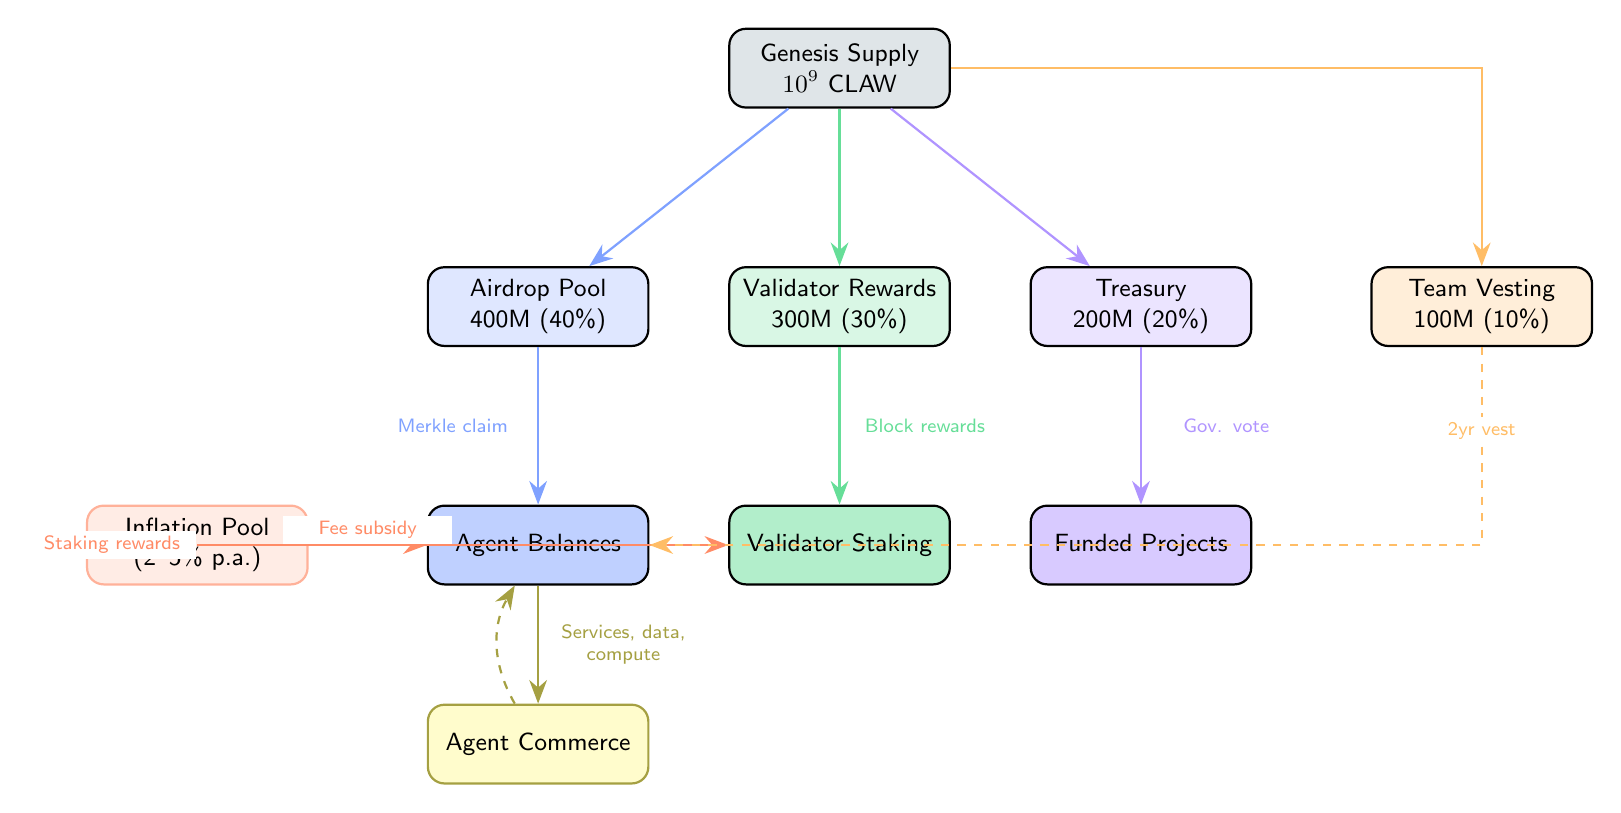
\begin{tikzpicture}[
    node distance=1.8cm,
    pool/.style={draw, rounded corners=6pt, minimum width=2.8cm, minimum height=1cm, font=\small\sffamily, thick, text width=2.5cm, align=center},
    flow/.style={-{Stealth[length=3mm]}, thick},
    label/.style={font=\scriptsize\sffamily, fill=white, inner sep=2pt, text width=2cm, align=center},
]

% Genesis
\node[pool, fill=clawgray!20] (genesis) {Genesis Supply\\$10^9$ CLAW};

% Distribution pools
\node[pool, fill=clawblue!15, below left=2cm and 1cm of genesis] (airdrop) {Airdrop Pool\\400M (40\%)};
\node[pool, fill=clawgreen!15, below=2cm of genesis] (validator) {Validator Rewards\\300M (30\%)};
\node[pool, fill=clawpurple!15, below right=2cm and 1cm of genesis] (treasury) {Treasury\\200M (20\%)};
\node[pool, fill=claworange!15, right=1.5cm of treasury] (team) {Team Vesting\\100M (10\%)};

% Agents and validators
\node[pool, fill=clawblue!30, below=2cm of airdrop] (agents) {Agent Balances};
\node[pool, fill=clawgreen!30, below=2cm of validator] (vals) {Validator Staking};
\node[pool, fill=clawpurple!30, below=2cm of treasury] (projects) {Funded Projects};

% Inflation
\node[pool, fill=clawred!10, draw=clawred!40, left=1.5cm of agents] (inflation) {Inflation Pool\\(2--5\% p.a.)};

% Commerce
\node[pool, fill=yellow!20, draw=yellow!60!black, below=1.5cm of agents] (commerce) {Agent Commerce};

% Flows
\draw[flow, clawblue!60] (genesis) -- (airdrop);
\draw[flow, clawgreen!60] (genesis) -- (validator);
\draw[flow, clawpurple!60] (genesis) -- (treasury);
\draw[flow, claworange!60] (genesis) -| (team);

\draw[flow, clawblue!60] (airdrop) -- node[label, left] {Merkle claim} (agents);
\draw[flow, clawgreen!60] (validator) -- node[label, right] {Block rewards} (vals);
\draw[flow, clawpurple!60] (treasury) -- node[label, right] {Gov. vote} (projects);

\draw[flow, clawred!60] (inflation) -- node[label, above] {Fee subsidy} (agents);
\draw[flow, clawred!60] (inflation) |- node[label, left, near start] {Staking rewards} (vals);

\draw[flow, yellow!60!black] (agents) -- node[label, right] {Services, data, compute} (commerce);
\draw[flow, yellow!60!black, dashed] (commerce) to[bend left=30] (agents);

% Team vesting arrow
\draw[flow, claworange!60, dashed] (team) |- node[label, above, near start] {2yr vest} (agents);

\end{tikzpicture}}% end resizebox
\caption{Complete CLAW token flow from genesis through distribution, staking, commerce, and inflation subsidy. Dashed arrows indicate time-locked or circular flows.}
\label{fig:tokenflow}
\end{figure}

\section{Formal Proofs: Extended}\label{app:proofs}

\begin{lemma}[Merkle Proof Soundness]
Given a collision-resistant hash function $\mathcal{H}$, the Merkle proof verification in Algorithm~\ref{alg:airdrop} (Phase~2) is sound: no agent can claim tokens not allocated to them unless $\mathcal{H}$ is broken.
\end{lemma}

\begin{proof}
Assume agent $i$ with DID $d_i$ and allocation $a_i$ submits a proof $\pi'$ claiming allocation $a' \neq a_i$. The leaf hash $\ell' = \mathcal{H}(d_i \| a')$. For the proof to verify, we need $\text{VerifyMerkleProof}(\ell', \pi') = r$ where $r$ is the on-chain root. But the root was computed from the true allocations $\{(d_j, a_j)\}$. Finding $\pi'$ such that verification succeeds with $\ell' \neq \ell_i$ requires finding a second preimage or collision in $\mathcal{H}$, contradicting collision resistance.
\end{proof}

\begin{lemma}[Governance Liveness]
Under the assumption that at least 50\% of total voting weight is held by non-Byzantine agents, the governance system maintains liveness: any valid proposal will eventually be decided.
\end{lemma}

\begin{proof}
Let $W_{\text{honest}} > 0.5 \cdot W_{\text{total}}$. Honest agents follow the protocol and vote on all proposals within the voting period. Since honest agents control majority weight, quorum ($>$50\% participation) is achievable. Given participation, majority voting produces a definitive yes/no outcome. Combined with the bounded voting period (14 days), every proposal terminates.
\end{proof}

\end{document}
